\documentclass{sig-alternate-05-2015}
\usepackage[utf8]{inputenc}
\usepackage[italian]{babel}
\usepackage[T1]{fontenc}
\usepackage{graphicx}
\usepackage{graphics}
\usepackage{listings}  
\usepackage{array}
\newcolumntype{L}[1]{>{\raggedright\let\newline\\\arraybackslash\hspace{0pt}}m{#1}}
\newcolumntype{C}[1]{>{\centering\let\newline\\\arraybackslash\hspace{0pt}}m{#1}}
\newcolumntype{R}[1]{>{\raggedleft\let\newline\\\arraybackslash\hspace{0pt}}m{#1}}
\usepackage{multirow}
\usepackage[table]{xcolor}
\usepackage{float}
\usepackage{array}
\usepackage{ragged2e}
\usepackage{cleveref}

\newcolumntype{P}[1]{>{\RaggedRight\hspace{0pt}}p{#1}}

\lstset{language=Java,tabsize=2,basicstyle=\ttfamily\scriptsize} 

\newcommand{\squeezeup}{\vspace{-0.5mm}}

\usepackage{etoolbox}
\makeatletter
\patchcmd{\@makecaption}
{\scshape}
{}
{}
{}
\makeatother

\newcolumntype{"}{@{\hskip\tabcolsep\vrule width 1pt\hskip\tabcolsep}}

\lstdefinestyle{base}{
	language=C,
	emptylines=1,
	breaklines=true,
	basicstyle=\ttfamily\color{black},
	moredelim=**[is][\color{red}]{@}{@},
}

\newcommand\FIXME[1]{\textbf{FIXME: #1}}

\begin{document}

% Copyright
\setcopyright{acmcopyright}
%\setcopyright{acmlicensed}
%\setcopyright{rightsretained}
%\setcopyright{usgov}
%\setcopyright{usgovmixed}
%\setcopyright{cagov}
%\setcopyright{cagovmixed}


%% DOI
%\doi{10.475/123_4}

%% ISBN
%\isbn{123-4567-24-567/08/06}

%Conference
\conferenceinfo{MSR '17}{May 20--21, 2017, Buenos Aires, Argentina}

%\acmPrice{\$15.00}

%
% --- Author Metadata here ---
%\conferenceinfo{WOODSTOCK}{'97 El Paso, Texas USA}
%\CopyrightYear{2007} % Allows default copyright year (20XX) to be over-ridden - IF NEED BE.
%\crdata{0-12345-67-8/90/01}  % Allows default copyright data (0-89791-88-6/97/05) to be over-ridden - IF NEED BE.
% --- End of Author Metadata ---

\title{Are We Reusing Outdated Code from Stack Overflow?}

\numberofauthors{1}
\author{
	\alignauthor
	$^1$Chaiyong Ragkhitwetsagul, $^1$Jens Krinke, $^2$Giuseppe Bianco \\
	\affaddr{$^1$University College London, London, UK}\\
	\affaddr{$^2$Università degli Studi del Molise, Campobasso, Italy}
}


\maketitle
\begin{abstract}
This paper provides a sample of a \LaTeX\ document which conforms,
somewhat loosely, to the formatting guidelines for
ACM SIG Proceedings. It is an {\em alternate} style which produces
a {\em tighter-looking} paper and was designed in response to
concerns expressed, by authors, over page-budgets.
It complements the document \textit{Author's (Alternate) Guide to
Preparing ACM SIG Proceedings Using \LaTeX$2_\epsilon$\ and Bib\TeX}.
This source file has been written with the intention of being
compiled under \LaTeX$2_\epsilon$\ and BibTeX.

The developers have tried to include every imaginable sort
of ``bells and whistles", such as a subtitle, footnotes on
title, subtitle and authors, as well as in the text, and
every optional component (e.g. Acknowledgments, Additional
Authors, Appendices), not to mention examples of
equations, theorems, tables and figures.

To make best use of this sample document, run it through \LaTeX\
and BibTeX, and compare this source code with the printed
output produced by the dvi file. A compiled PDF version
is available on the web page to help you with the
`look and feel'.
\end{abstract}

\section{Introduction}
%The popularity of the Internet encourages tremendous amount of source code being shared online. 
Stack Overflow is a popular online programming community with 6.3 million users. It allows programmers to ask questions and give answers to programming problems. The website has found to be useful for software development and also valuable for educational purposes \cite{x}. On Stack Overflow, each conversation contains a question and answer(s).  The answers normally contain at least one code snippet as a solution to the question asked. The code snippet is usually not written directly on Stack Overflow website but copied from another location. It can be copied and modified from the problematic code snippet in the question, copied from an answerer's own code, or borrowed from other locations including open source software (OSS) systems. As a result, the process of posting and answering questions on Stack Overflow which involves copying and pasting source code can be considered as code cloning. 

Code cloning is an activity of reusing source code by copying and pasting. It normally occurs in software development and account from 7\% to 23\% in typical software systems \cite{Bellon2007}. The benefits and drawbacks of clones are still controversial. Several authors state that clones lead to bug propagations and software maintenance issues \cite{Kamiya2002}, while some others have proofs that in some cases clones are not harmful than normal code or even beneficial \cite{Saini2016,Kapser2006}. Code cloning can also have side effects of violating software licenses. Carelessly cloning code from one project and reusing it in another project with different license may cause software licensing violation \cite{German2009}.

In this study, we treat code snippets that are copied from software systems to Stack Overflow, and vice versa, as code clones. We call them \textbf{online code clones}. There are three ways to create online code clones: (1) code is cloned from a software project to Stack Overflow as an example; (2) code is cloned from Stack Overflow to a software project to obtain a functionality, perform a particular task, or fixing a bug; and (3) code is implicitly cloned from one software project to another by having Stack Overflow as a medium. Online code clones can similarly lead to a problem of bug propagation as classical code clones. Unfortunately, they are more difficult to locate and fix since the search space from online corpora is larger and no longer confined in a local repository.

A motivating example of problems caused by online code clones can be found in a Stack Overflow post regarding how to implement RawComparator in Hadoop\footnote{http://stackoverflow.com/questions/22262310}. In \Cref{fig:before-after}, the left hand side shows a code snippet embedded as a part of accepted answer to the question. The snippet shows how Hadoop implements \textit{compare} method in its \textit{WritableComparator} class. The code snippet on the right hand side shows another version of the same \textit{compare} method in \textit{WritableComparator} class but it is extracted from the latest version of Hadoop. We can obviously see that they are highly similar except one line, \verb|buffer.reset(null,0,0);|, added in the latest version after \verb|key2.readFields(buffer);|. The added line is intended for cleaning up the reference in \verb|buffer| variable. While this change has already been introduced into \textit{compare} method in the latest version of Hadoop, the code example in Stack Overflow post is still unchanged and outdated. This example shows that there can be inconsistencies between online code clones and its original.  %Since reusing source code from Stack Overflow is considered a common practice nowadays, the scale of online code cloning is more than intra or inter project clone in a local code bases. 
This is an emerging and challenging problem. Since studies in this area are still limited, we aim to gain more insight of the problem in this study. %We are interested to gain more insights of online code clone in this study.

\begin{figure*}
\begin{lstlisting}
/* Code in Stack Overflow #22315734 */                      /* WritableComparator.java (2016-09-26) */
1 public int compare (byte[] b1,int s1,int l1,              1 public int compare(byte[] b1,int s1,int l1,
2                     byte[] b2,int s2,int l2) {            2                    byte[] b2,int s2,int l2) {
3   try {                                                   3   try {
4     buffer.reset(b1,s1,l1); /* parse key1 */              4     buffer.reset(b1,s1,l1); /* parse key1 */
5     key1.readFields(buffer);                              5     key1.readFields(buffer);
6     buffer.reset(b2,s2,l2); /* parse key2 */              6     buffer.reset(b2,s2,l2); /* parse key2 */
7     key2.readFields(buffer);                              7     key2.readFields(buffer);
8   } catch (IOException e) {                               8     buffer.reset(null,0,0); /* clean up reference */
9     throw new RuntimeException(e);                        9   } catch (IOException e) {
10   }                                                      10    throw new RuntimeException(e);
11   return compare(key1,key2); /* compare them */          11  }
12 }                                                        12  return compare(key1, key2); /* compare them */
                                                            13 }
\end{lstlisting}
\caption{The same code fragments, WritableComparator.java, on Stack Overflow post 22315734 and latest version in hadoop code base}
\label{fig:before-after}
\end{figure*}

This paper makes the following  primary contributions:

\vspace{0.5ex}%
\noindent\textbf{1.~A manual study of online code clones:} 
We used two clone detection tools to discover 266,837,480 similar code fragment pairs and manually investigated 7,840 candidate clone pairs between Java code fragments obtained from Stack Overflow accepted answers and 109 Java open source projects.

\vspace{0.5ex}%
\noindent\textbf{2.~Addressing the problems of reusing source code between open source projects and Stack Overflow:} Our study shows that there are at least 238 clones that have been obviously copied from open source projects or external online sources to Stack Overflow as code examples which potentially violate their software licenses. Furthermore, 50 out of the 84 clones are outdated and questionable for being reused.

\section{Empirical Study}
We perform an empirical study of online code clones between Stack Overflow and 109 Java open source projects to answer the following research questions: \\ 
\textbf{RQ1 (online code clones):} \textit{To what extent  source code is cloned between Stack Overflow and open source projects?} We would like to quantitatively measure the number of online code clones between Stack Overflow and open source projects to understand the scale of the problem. \newline
%\textbf{RQ2 (flow of online code clones):} \textit{what are the directions that source code is cloned?} If clones between the two locations exist, we would like to observe in which direction the code has been copied. Is it mostly from Stack Overflow to open source projects, or the other way around, or equally both? \newline
\textbf{RQ2 (classification of online code clones):} \textit{What are the main characteristics among the set of online code clones?} We group them into seven groups according to our pre-defined classification scheme so we can differentiate and understand the motivation of cloning. Some of the clones are copy from open source projects to Stack Overflow, while some are copied from a third-party location, and some are accidental clones containing boiler-plate code, and code stubs generated by IDE. \newline
\textbf{RQ3 (effects of online code clones):} \textit{what are the effects derived from online code clones? can they be harmful to software development?} Is there observable problems caused by clones between Stack Overflow and open source projects?

\begin{figure*}
	\centering
	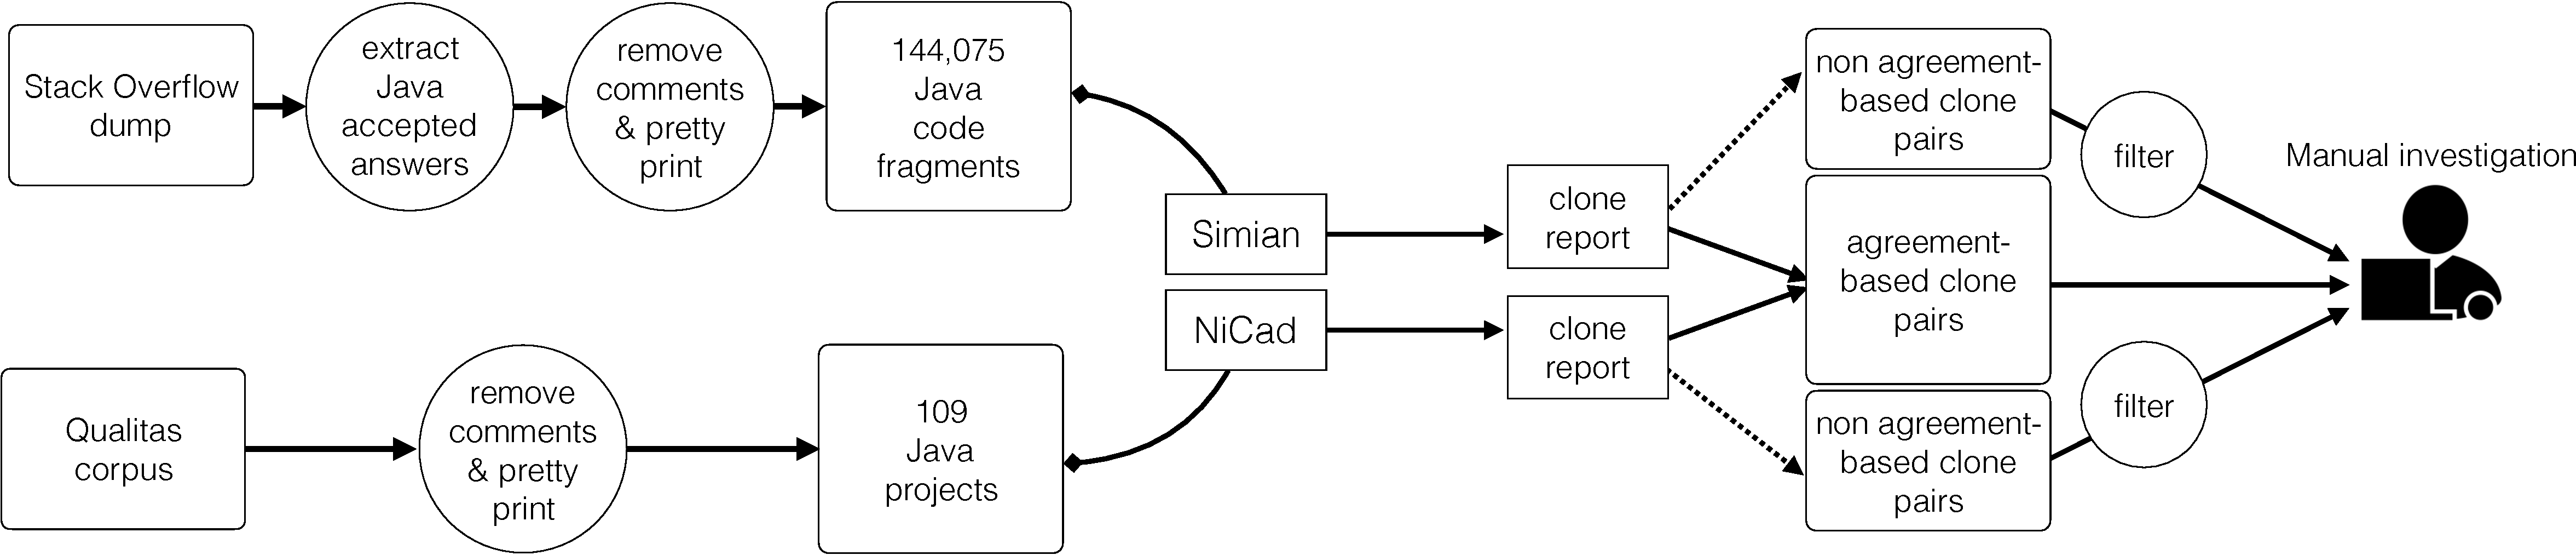
\includegraphics[width=0.9\linewidth]{exp_framework}
	\caption{Experimental framework}
	\label{fig:exp_framework}
\end{figure*}

\subsection{Experimental Framework}
To answer the three research questions, an experimental framework is designed as depicted in \Cref{fig:exp_framework}. We process two datasets, Stack Overflow and open source projects from Qualitas corpus. Java code fragments are extracted from Stack Overflow posts using regular expressions. We pre-process Java code in both datasets by removing comments and pretty-printing to increase accuracy of clone detection. Then, we deploy two clone detection tools, Simian \cite{simian} and NiCad \cite{Roy2008,Cordy}, to locate clones between the two datasets. Due to a technical limit of Simian and NiCad to scale to large datasets, we partition the input and run the tools multiple times. Each run is composed of the whole Stack Overflow data and a single Qualitas project. We repeat the process until we cover 111 projects. 

We then convert the clone reports to General Clone Format (GCF)~\cite{Wang2013} and combine them into a single file. GCF provides a common format for clones which enable us to reuse scripts that analyse clone reports from Simian and NiCad. Moreover, using GCF, other additional clone detectors can be adopted, if needed, without any changes in the analysis. Simian do not provide an option to detect inter clones between two locations. Hence the Simian GCF clone report is pruned to contain only inter clone pairs between Stack Overflow and Qualitas project. In this step, all intra clone pairs within Stack Overflow and open source projects are removed. NiCad provides an option to detect inter clones so no pruning is needed. Next, clone pairs reported from the two clone detectors are pair-wise matched to find agreements using Bellon's clone overlapping criteria \cite{Bellon2007}. This step generates \textbf{agreement-based clone pairs}. They are clones with highest confidence since they receive agreement from both tools. Then, clone pairs reported by Simian and NiCad that do not find agreement are filtered by size of minimum 10 lines. This step generates \textbf{non agreement-based clone pairs}. The non agreement-based clone pairs are clones with less confidence than agreement-based ones. Finally, agreement-based and non agreement-based clone pairs are looked at and classified manually by the first author.

In the manual inspection process, we classify clones into categories according to their properties. This process takes approximately a months until we successfully classified 7,840 clone pairs into categories. Some of the clone candidates are false clones due to being boiler-plate code or IDE-generated and are discarded for further analysis. By ignoring the false clones, we compare licensing information of 477 remaining clone pairs for possibility of software licensing violations. Moreover, we look forward through history of the clones from the projects' git versioning systems. This is to see if there is any changes made to the clones after it has been copied, hence resulting in outdated clones on Stack Overflow.

\subsection{Experimental Setup}

\subsubsection{Datasets}
\begin{table}
	\centering
	\caption{Stack Overflow and Qualitas datasets}
	\label{tab:datasets}
	\small
	\begin{tabular}{l|r|r}
		\hline 
		Dataset & No. of files & SLOC \\
		\hline
		Stack Overflow & 144,075 & 2,347,269 \\ 
		\hline 
		Qualitas &  160,937 & 19,086,883 \\ 
		\hline 
	\end{tabular} 
\end{table}

\textbf{Stack Overflow}: we extracted Java code snippets from accepted answers in a snapshot of Stack Overflow dump \footnote{https://archive.org/details/stackexchange} in January 2016. The archived dump has a size of 9 gigabytes. The data dump is in XML format containing information of \textit{Posts} (questions and answers) and supporting data such as user accounts and timestamps of the posts. We are interested in code snippets embedded in posts which are pieces of code located between \texttt{<code></code>} tags. We filtered the snippets with two filtering criteria. First, we ignore snippets that are less than 6 lines since they are usually not considered as clones by clone detection research \cite{something}. Second, we are only interested in code snippets from posts that are marked accepted answer since they have high chances to be reused than snippets in questions and other answers. Each snippet is extracted from the dump using regular expressions and saved to a file using its post ID as the file's name. We use \texttt{.java} extension so that the clone detectors can recognise them. If a Stack Overflow conversation has more than one code snippet in the accepted answer, we append an indexing number starting from zero after the post ID (e.g. 45051109\_0.java, and 45051109\_1.java). With the two filters, we finally obtained 144,075 Java code snippets which contain xxx lines of Java source code excluding comments and blank lines\footnote{measured by cloc: https://github.com/AlDanial/cloc}.

\textbf{Open source systems}: we selected an established corpus for an empirical software engineering study called \textbf{Qualitas} \cite{QualitasCorpus}. It is a curated Java corpus that has been used in several software engineering studies \cite{Taube-Schock2011,Beckman2011,Vasilescu2011,Omar2012}. The projects in the corpus represent various domains of software systems ranging from programming language to 3D and visualisation \cite{QualitasCorpus}. We selected the 20130901r snapshot of Qualitas corpus containing 112 Java open source projects. This release contains projects with releases no later than 1st September 2013. We chose a snapshot late back in 2013 since we are interested in online code clones in the direction from open source projects to Stack Overflow. The 20130901r snapshot provides Java code that is at least 3 years old from the time of the experiment, January--December 2016. The time difference is sufficiently long for a number of code snippets to be copied onto Stack Overflow. Out of 112 Qualitas projects, there is one project, \textit{jre}, that does not contain Java source code so it is removed from the study. This results in totally 111 projects analysed in the study. As shown in \Cref{tab:datasets}, the 111 Qualitas project have 160,937 Java files containing 19,086,883 lines of code. %Details of the 109 Qualitas projects and their licenses are listed in Table \ref{t:new_and_old}.

\subsubsection{Clone Detectors}
There is a number of restrictions in terms of choosing clone detection tools for this study. Firstly, they have to support Java. Secondly, due to nature of code snippets posted on Stack Overflow, some of them are not complete Java classes or methods. Hence, the tool must be flexible enough to process code snippets that are neither a complete block nor compilable. Thirdly, since the amount of code that have to be processed are in a scale of millions line of code (as shown in \Cref{tab:datasets}), a clone detector must be scalable enough to successfully complete the execution and report clones in a reasonable amount of time. We have tried running 5 state-of-the-art clone detectors including Simian \cite{simian}, NiCad \cite{Cordy,Roy2008}, CCFinder \cite{Kamiya2002}, iClones \cite{Gode2009}, and DECKARD \cite{Jiang2007a} against Stack Overflow and Qualitas datasets. CCFinder, iClones, and DECKARD failed to successfully detect clones between 144,075 Stack Overflow code snippets and 109 Qualitas projects. All of them reported execution errors after running for couple of hours. Thus, we removed them from the study. Simian and NiCad completed the detection with success. We found that both of them are also flexible enough to handle million-SLOC code corpus with method or class incompleteness. So, we decided to use both of them.

\textbf{Simian} is a text-based clone detector which locate clones at line-level granularity and has been used extensively in several clone studies \cite{Ragkhitwetsagul2016, Wang2013, Mondal2011, Cheung2015, Krinke2010}. It is a command-line tool which enables us to automate the detection. Furthermore, it offers normalisation of variable names and literals (strings, and numbers) which enable Simian to detect clones of type 1 and type 2. \textbf{NiCad} is also a text-based clone detector which detects clones at either method- or block-level granularity. It can detect clones up to type 3 and is used in several clone studies \cite{Roy2008, Ragkhitwetsagul2016, Svajlenko2014, Wang2013, Mondal2011, Sajnani2016}. It utilises TXL for parsing and pretty-printing source code. It also provide code normalisation by variable renaming and code abstraction. We use a variant of NiCad called \textit{nicadcross}. It offers the same functionalities as the original NiCad but is specialised for detecting code clones between two systems. NiCad is also a command-line tool which makes it suitable for automation.

\subsubsection{Agreement-based Clone Filtering}
The number of detected clones between two datasets  can be very large. In our study, there are totally 266,837,480 clone pairs reported. It is infeasible for human to manually validate all of them. One can do sampling of clones from this huge clone pair set. However, they may end up having most of them false positive clones. Therefore, we adopted an idea of clone agreement which has been used in clone research studies \cite{Wang2013,Funaro2010,cr2016ssbse} in a situation that clone oracle is missing or impossible to establish. Clone pairs agreed by multiple clone detection tools have higher confident to be real clones \cite{cr2016ssbse}. By using this agreement-based clone detection approach, we can reduce the number of clone candidates for manual investigation by paying more attention to the ones agreed by multiple tools. To find agreement of two clone pairs, we resort to an approach proposed in a study by Bellon et al.~\cite{Bellon2007}. Two clone pairs which have large enough overlapping clone lines can be categorised as either a good-match or an ok-match pair. A good-match clone pair has stronger agreement than an ok-match pair. We follow the same following definitions introduced in the original paper.

%good and ok-match clone pairs are defined as follows. 
A clone pair \textit{CP} is formed by two clone fragments \textit{CF$_1$} and \textit{CF$_2$} with a pre-defined similarity threshold \textit{t}, i.e. \textit{CP} = (\textit{CF$_1$}, \textit{CF$_2$}, \textit{t}).  We can define \textit{overlap} and \textit{contained} value of two clone pairs as 
%\squeezeup
\begin{multline}
	overlap(\textrm{\textit{CP}}_1, \textrm{\textit{CP}}_2) = \frac{|lines(\textrm{\textit{CF}}_1) \cap lines(\textrm{\textit{CF}}_2)|}{|lines(\textrm{\textit{CF}}_1) \cup lines(\textrm{\textit{CF}}_2)|} 
\end{multline}
%\squeezeup
\begin{multline}
	contained(\textrm{\textit{CP}}_1, \textrm{\textit{CP}}_2) = \frac{|lines(\textrm{\textit{CF}}_1) \cap lines(\textrm{\textit{CF}}_2)|}{|lines(\textrm{\textit{CF}}_1)|}. 
\end{multline}

\textit{good-value} of two clone pairs is then defined as
%\squeezeup
\begin{align*}
	good(\textrm{\textit{CP}}_1, \textrm{\textit{CP}}_2) = min(overlap(\textrm{\textit{CP}}_1.\textrm{\textit{CF}}_1,\textrm{\textit{CP}}_2.\textrm{\textit{CF}}_1), \\ overlap(\textrm{\textit{CP}}_1.\textrm{\textit{CF}}_2,\textrm{\textit{CP}}_2.\textrm{\textit{CF}}_2)).
\end{align*}

\textit{ok-value} is defined as
%\squeezeup
\begin{align*}
	ok(\textrm{\textit{CP}}_1,\textrm{\textit{CP}}_2) = min(max(contained(\textrm{\textit{CP}}_1.\textrm{\textit{CF}}_1,\textrm{\textit{CP}}_2.\textrm{\textit{CF}}_1), \\ contained(\textrm{\textit{CP}}_2.\textrm{\textit{CF}}_1,\textrm{\textit{CP}}_1.\textrm{\textit{CF}}_1)),
	\\ max(contained(\textrm{\textit{CP}}_1.\textrm{\textit{CF}}_2,\textrm{\textit{CP}}_2.\textrm{\textit{CF}}_2), \\contained(\textrm{\textit{CP}}_2.\textrm{\textit{CF}}_2,\textrm{\textit{CP}}_1.\textrm{\textit{CF}}_2))).
\end{align*}

Two clone pairs $\textrm{\textit{CP}}_1$ and $\textrm{\textit{CP}}_2$ are called a \textit{good-match(p)} iff, for $p \in [0,1]$ holds 
%\squeezeup
\begin{equation}
good(\textrm{\textit{CP}}_1,\textrm{\textit{CP}}_2) \geq p.
\end{equation}

Similarly for an \textit{ok-match(p)} pair
%\squeezeup
\begin{equation}
ok(\textrm{\textit{CP}}_1,\textrm{\textit{CP}}_2) \geq p.
\end{equation}

Using this good-match and ok-match criteria with a predefined threshold \textit{p}, we can prune the 266-million candidate clone pairs for manual investigation. good-match pairs are the ones with the highest confident and ranked the first to be looked at, followed by ok-match pairs, and followed by clone pairs without agreement.

\subsection{Clone detectors' parameter tuning}
We are aware of effects of configurations to clone detection results and the importance of searching for optimised configurations in empirical clone studies \cite{Wang2013,cr2016ssbse,Ragkhitwetsagul2016,Svajlenko2014}. However, considering the size of the two datasets and search space of at least 15 Simian's and 5 NiCad's parameters, we are hindered from searching for the best configurations of the tools. Thus, we decided to configure Simian and NiCad using two established configurations: 1) the tools' default configurations chosen by the tools' creators (denoted as \textit{df}), and 2) the discovered configurations for Bellon's Java projects from \textit{EvaClone}, a study of optimising clone detectors' configurations based on clone agreement, by Wang et al.~\cite{Wang2013} (denoted by \textit{EvCl}). The details of the two configurations are described in \Cref{t:param_tuning}. Having two clone detectors multiplied by two chosen configurations, we look for agreements in four possible pair-wise combinations: Simian$_{df}$--NiCad$_{df}$, Simian$_{df}$--NiCad$_{\textrm{\textit{EvCl}}}$, Simian$_{\textrm{\textit{EvCl}}}$--NiCad$_{df}$, and Simian$_{\textrm{\textit{EvCl}}}$--NiCad$_{\textrm{\textit{EvCl}}}$.

\begin{table}
	\centering
	\caption{Configurations of Simian and NiCad}
	\label{t:param_tuning}
	\resizebox{\columnwidth}{!}{%
		\scriptsize
\begin{tabular}{l|p{5.5cm}}
	\hline 
	Tool & Parameters \\
	\hline
	Simian$_{\textrm{\textit{df}}}$ &  threshold=6, ignoreStringCase, \newline ignoreCharacterCase, ignoreModifiers \\ 
	\hline
	Simian$_{\textrm{\textit{EvCl}}}$ & threshold=5, ignoreIdentifiers, \newline ignoreIdentifierCase, ignoreStrings, \newline ignoreCharacters, ignoreSubtypeNames, \newline balanceSquareBrackets  \\ 
	\hline 
	NiCad$_{\textrm{\textit{df}}}$ & MinLine=10, MaxLine=1000, UPI=0.30 \\
	\hline
	NiCad$_{\textrm{\textit{EvCl}}}$ & MinLine=5, MaxLine=604, UPI=0.20, \newline blind renaming, literal abstraction \\ 
	\hline 
\end{tabular} %
}
\end{table}

\section{Results}

\begin{table}
	\centering
	\caption{Statistics of clones found between Stack Overflow and Qualitas projects using Simian and NiCad}
	\label{tab:raw_stats}
	\small
	\resizebox{\columnwidth}{!}}}$ & 29\% & 28\% & 25\% & 21\% \\
			\hline
		\end{tabular} %
	}
\end{table}

The clone statistics obtained from running Simian and NiCad with \textit{df} and \textit{EvCl} configurations are presented in \Cref{tab:raw_stats}. Preliminary manual investigation of Simian's clone report revealed that there were problematic 11 fragments. These 11 fragments trigger Simian to generate large clone clusters containing a huge number of false clones of array initialisation. Hence, they were removed from Simian's clone reports before the analysis. From \Cref{tab:raw_stats}, Simian clones cover approximately 10\% of the 144,075 Stack Overflow snippets, 1,406 reported by Simain$_{df}$ and 1,360 from Simain$_{\textrm{\textit{EvCl}}}$ respectively. NiCad$_{df}$ reports clones in 1,197 Stack Overflow code snippets, while NiCad$_{\textrm{\textit{EvCl}}}$ reports clones in a larger number of 12,884 snippets  mainly due to its relaxed configurations. In terms of number of clone pairs, Simian$_{\textrm{\textit{EvCl}}}$ and NiCad$_{\textrm{\textit{EvCl}}}$ report an enormous number of clone pairs of 59,936,722 and 206,718,663 respectively. This is expected since EvaClone configurations prefer recall \cite{Wang2013}. The average clone size of Simian$_{df}$ is 7.45 lines which is bigger than its Simian$_{\textrm{\textit{EvCl}}}$ counterpart of 4.81. Similarly, NiCad$_{df}$ has an average clone size of 9.54 lines which is bigger than 5.31 reported by NiCad$_{\textrm{\textit{EvCl}}}$. We can see from the statistics that EvaClone tunes the tools in the way that they report smaller clones. The average percentage of Stack Overflow code snippets that are cloned according to Simian$_{df}$, Simian$_{\textrm{\textit{EvCl}}}$, NiCad$_{df}$, and NiCad$_{\textrm{\textit{EvCl}}}$ is 28\%, 29\%, 25\%, and 21\% accordingly.

\begin{table}
	\centering
	\caption{No.~of projects in Qualitas successfully analysed by Simian and NiCad}
	\label{tab:projects_missing}
	\small
	\begin{tabular}{l|r|r|r|r}
		\hline
		& Simian$_{\textrm{\textit{df}}}$ & Simian$_{\textrm{\textit{EvCl}}}$  & NiCad$_{\textrm{\textit{df}}}$ & NiCad$_{\textrm{\textit{EvCl}}}$ \\ 
		\hline
		\textit{Successful} & 111 & 111 & 105 & 84 \\ 
		\textit{Clust.~fail} & -- & -- & 6 & 16 \\
		\textit{Renm.~fail} & -- &  -- & -- & 11 \\
		\hline
	\end{tabular}
\end{table}



%\begin{table*}[h]
%	\centering
%	\caption{Statistics of clones found between Stack Overflow and Qualitas projects using Simian and NiCad}
%	\label{tab:raw_stats}
%%	\resizebox{\columnwidth}{!}{%
%	\small
%		\begin{tabular}{l|r|r|r|r|r|r|r|r|r|r|r|r}
%			\hline
%			\multirow{3}{*}{Statistics} 
%			& \multicolumn{3}{c|}{Simian$_{df}$} 
%			& \multicolumn{3}{c|}{Simian$_{\textrm{\textit{EvCl}}}$}
%			& \multicolumn{3}{c|}{NiCad$_{df}$} 
%			& \multicolumn{3}{c}{NiCad$_{\textrm{\textit{EvCl}}}$} \\ \cline{2-13} 
%			& \multicolumn{3}{c|}{1406 fragments} 
%			& \multicolumn{3}{c|}{1360 fragments}  
%			& \multicolumn{3}{c|}{1197 fragments} 
%			& \multicolumn{3}{c}{12884 fragments} \\ \cline{2-13}
%			& $C_{\mathrm{pairs}}$ & $C_{\mathrm{SLOC}}$ & $C_{\mathrm{\%}}$ 
%			& $C_{\mathrm{pairs}}$ & $C_{\mathrm{SLOC}}$ & $C_{\mathrm{\%}}$ 
%			& $C_{\mathrm{pairs}}$ & $C_{\mathrm{SLOC}}$ & $C_{\mathrm{\%}}$
%			& $C_{\mathrm{pairs}}$ & $C_{\mathrm{SLOC}}$ & $C_{\mathrm{\%}}$ \\ 
%			\hline
%			Total & 54790 & -- & -- 		& 59936722 & --	& -- 		& 127305 	& -- & -- 	& 206718663 & -- & -- \\
%			Mean & 52 & 7.45 & 28\% 		& 44104 & 4.81 & 29\% 		& 106 & 9.54 & 25\% 	& 16046 & 5.31 & 21\% \\
%			Std Dev. & 147 & 3.22 & 23\% 	& 1040483 & 1.20 & 19\% 	& 209 & 3.10 & 18\% 	& 21890 & 1.92 & 16\% \\
%			Max  & 1020 & 49.00 & 94\% 		& 38223637 & 18.00 & 89\% 	& 2100 & 39.00 & 81\% 	& 442655 & 50.00 & 93\% \\
%			Min  & 1 & 5.00 & 1\% 			& 1 & 4.00 & 2\% 			& 1 & 7.00 & 2\% 		& 1 & 3.00 & 1\% \\
%			Median  & 3 & 7.00 & 21\% 		& 24 & 5.00 & 25\% 			& 20 & 8.00 & 19\% 		& 8003 & 5.00 & 16\% \\
%			Mode  & 1 & 7.00 & 33\% 		& 1 & 4.00 & 50\% 			& 1 & 8.00 & 67\% 		& 1 & 4.00 & 33\% \\
%			\hline
%		\end{tabular} %
%%	}
%\end{table*}

%\begin{table*}
%	\centering
%	\caption{109 Qualitas projects (new versions retrieved on 2016-09-27)}
%	\label{t:new_and_old}
%%	\resizebox{\columnwidth}{!}{%
%	\small
%		\begin{tabular}{l|r|r|c|c|p{3cm}|p{3cm}}
%			\hline 
%			Projects & Old version & New versions & Latest change & CVS & License & Notes \\
%			\hline
%			antlr4 & 4.0 & 4.5.4 & 25/09/2016 & git & BSD & \\
%			apache-ant & 1.8.4 & 1.10.0 & 09/04/2016 & git & Apache2.0 & \\
%			argouml & 0.34 & 0.35.4 & 11/01/2015 	& svn & Eclipse  1.0 & \\
%			artofillusion & 2.8.1 & 3.0.2 & 27/08/2016 & svn & GPL 2.0 & \\
%			aspectj & 1.6.9 & 1.8.9 & 12/05/2016 & git & Eclipse   1.0 & \\
%			axion & 1.0-M2 & - & 08/03/2013 & - & Proprietary (BSD/Apache-style) & \\
%			batik & 1.7 & 1.9.0 & 11/05/2016 & svn & Apache , v.2.0 & \\
%			c-jdbc & 2.0.2 & - & 16/09/2005 & - & GLGPL 2.1 & \\
%			castor & 1.3.1 & 1.4.2 & 17/08/2016 & git & Apache 2.0 & \\
%			cayenne & 3.0.1 & 4.0.M4 &  26/09/2016 & git & Apache 2.0 & \\
%			checkstyle & 5.1 & 7.2  & 23/09/2016 & git & GLGPL 2.1 \& Apache 2.0 & \textit{Cli, Logging and Beanutils} packages are from the Apache Commons project. \\
%			cobertura & 1.9.4.1 & 2.1.2 & 01/06/2016 & git & GPL 2.0  & \\
%			colt & 1.2.0 & - & 09/09/2014 & - & Proprietary (CERN) & Found multithreaded v. \\
%			columba & 1.4 & - & 20/04/2007 & - & Mozilla   1.1  & \\
%			commons-collections & 3.2.1 & 4.2 & 12/09/2016 & svn & Apache 2.0 & \\
%			compiere & 330 & - & - & - & GPL 2.0 & No longer OSS \\
%			db-derby & 10.6.1.0 & 10.12.1 & 13/08/2016 & svn & Apache 2.0 & \\
%			displaytag & 1.2 & 2.0 & 17/08/2014 & svn & MIT  & \\
%			drawswf & 1.2.9 & - & 02/04/2013 & - & GPL 2.0 & \\
%			drjava & 20100913-r5387 & ??? & 03/09/2014 & svn & BSD  & Build to see version? \\
%			exoportal & ??? & ??? &  & git & GLGPL 3.0 \& proprietary & Too many new projects \\
%			emma & 2.0.5312 & 2.0.5312 & 09/05/2013  & - & Common   1.0 & \\
%			findbugs & 1.3.9 & 3.0.1 & 06/03/2015 & - & GLGPL 2.0 & \\
%			fit-java & 1.1 & - & 04/06/2013 & - & GPL 2.0 & \\
%			fitlibrary & 20100806 & ??? & 29/07/2014 & git & GPL 2.0 & \\
%			freecol & 0.10.7 & 0.11.6 & 26/09/2016 & git & GPL 2.0 &  \\
%			freecs & 1.3.20100406 & - & 22/04/2013 & - & GPL 3.0 &   \\
%			freemind & 0.9.0 & 1.0.0 & 16/08/2016 & git & GPL 2.0+ &  \\
%			galleon & 2.3.0 & 2.5.6 & 29/04/2013 & - & GPL 2.0 & \\
%			ganttproject & 2.0.9 & 2.8.1 & 16/08/2016 & git & GPL 3.0 &  \\
%			geotools & 2.7-M3 & 16 & 27/09/2016 & git & GLGPL 2.0 & \\
%			hadoop & 1.0.0 & 3.0.0-alpha2 & 26/09/2016 & git & Apache 2.0 & \\
%			heritrix & 1.14.4 & - & 05/06/2013 & - & GLGPL 2.1 & \\
%			hibernate & 4.2.2 & 5.2.3 & 22/09/2016 & git & GLGPL 2.1+ & \\
%			hsqldb & 2.0.0 & 2.3.4 & 13/09/2016 & svn & BSD  & \\
%			htmlunit & 2.8 & 2.24 & 26/09/2016 & svn & Apache 2.0 & \\
%			ireport & 3.7.5 & - & 28/05/2014 & - & Affero GLGPL 3.0 & \\
%			itext & 5.0.3 & 5.5.9 & 27/09/2016 & git & Affero GLGPL 3.0 & \\
%			informa & 0.7.0-alpha2 & - & 07/11/2008 & - & GLGPL 2.1 \& Apache Software 1.1 & \\
%			ivatagroupware & 0.11.3 & - & 27/02/2013 & - & GPL 2.0 & \\
%			jfin\_datemath & R1\_0\_1 & - & 25/04/2013 & - & GPL 2.0 & \\
%			joggplayer & 114s & - &  15/04/2013 & - & GPL 2.0 & \\
%			jag & 6.1 & 6.2 & 08/04/2013  & - & GPL 2.0 \& BSD  & BSD  is for libraries. \\
%			james & 2.2.0 & 2.3.2.1 & 14/08/2015 & - & Apache 2.0 & \\
%			jasml & 0.10 & - & 08/03/2013 & - & Apache Software  & \\
%			jasperreports & 3.7.4 & 6.3.1 & 27/09/2016 & git & GLGPL 3.0 &  \\
%			javacc & 5.0.0 & 7.0.0 & 15/08/2016 & svn & Proprietary (Sun) & \\
%			jboss (wildfly) & 5.1.0.GA & 11.0.0.Alpha1 & 27/09/2016 & git & GLGPL 2.1 & Renamed to Wildfly. \\
%			jchempaint & 3.0.1 & 3.4 & 01/09/2016 & git & GLGPL 2.1+ &  \\
%			jedit & 4.3.2 & 5.3.1 & 20/09/2016 & svn & GPL 2.0 &  \\
%			jena & 2.6.3 & 3.1.1 & 16/09/2016 & git & Apache 2.0 & \\
%			jext & 5.0 & - & 18/08/2004 & - & GPL 2.0 &  \\
%			jfreechart & 1.0.13 & 1.5.0 & 29/08/2016 & git & GLGPL 2.0 &   \\
%			jgraph & 5.13.0.0 & 3.6.0.0 & 07/09/2016 & git & Proprietary (mxGraph) & \\
%			jgraphpad & 5.10.0.2 & - & 10/11/2006 & - & GPL   \& GLGPL (derivatives) & \\
%			jgrapht & 0.8.1 & 1.0.1 & 23/09/2016 & git & GLGPL 2.1 \& Eclipse  1.0 & \\
%			jgroups & 2.10.0.GA & 4.0.0 & 26/09/2016 & git & Apache 2.0 & \\
%			jmoney & 0.4.4 & ??? & 27/12/2015 & git & GPL 2.0 &  \\
%			jparse & 0.96 & - & 29/07/2004 & - & GLGPL 2.1 & \\
%			jpf & 1.5.1 & ??? & 13/01/2012 & - & Apache 2.0 & \\
%			junit & 4.11 & 4.12 & 04/12/2014 & git & Eclipse  1.0 & \\
%			shiftone-jrat & 0.6 & 1-beta-1 & 17/11/2007 & svn & GLGPL 2.0 &  \\
%			vuze & 4812 & 5730 & 23/09/2016 & svn & GPL 2.0 & \\
%			\hline
%		\end{tabular} %
%%	}
%\end{table*}

\begin{table}
	\centering
	\caption{13 Qualitas projects that have been cloned as examples on Stack Overflow with their respective licenses}
	\label{t:new_and_old}
	%	\resizebox{\columnwidth}{!}{%
	\small
	\begin{tabular}{l|r|p{4cm}}
		\hline 
		Project & Version & Licenses (no.~of files) \\
		\hline
%		apache-ant & 1.8.4 & Apache2.0 \\
%		apache-log4j & 1.2.16 & \\
		aspectj & 1.6.9 & Apache-1.1 (182), CPLv1 (3), \newline EPLv1 (2011), None (23), \newline SeeFile (6), Unknown (286) \\
		\hline
		hadoop & 1.0.0 & Apache-2 (1,935), \newline spxdBSD/Apache-2 (8) \newline None (33), Unknown (14) \\
		\hline
		hibernate & 4.2.2 & Apache-2 (20), \newline GLGPLv2.1+ (31) \newline PublicDomain (1), \newline None (1,850), SeeFile (4), \newline Unknown (4,324) \\
		\hline
		jasperreports & 3.7.4 & GLGPLv2.1+ (3), \newline GLGPLv3+ (1,581), \newline None (1), Unknown (4)\\
		\hline
		jfreechart & 1.0.13 & GLGPLv2.1+ (989) \\
		\hline
		jgraph & 5.13.0.0 & GLGPLv2.1+ (4), \newline spdxBSD (2), Unknown (151), \newline None (24), SeeFile (9) \\
		\hline
%		jgrapht & 0.8.1 & GLGPL 2.1 \& Eclipse  1.0 \\
		jstock & 1.0.7c & GLGPLv2.1+ (1), \newline GPLv2+ (239), \newline Apache-2 (1), BSD3 (1), \newline None (23), SeeFile (1), \newline spdxMIT (3), Unknown (5)\\
		\hline
		jung2 & 2-0-1 & N/A \\
		\hline
		junit & 4.11 & None (160), Unknown (4)  \\
		\hline
		poi & 3.6 & Apache-2 (2,002), None (5) \\
		\hline
		spring & 3.0.5 & Apache-2 (2,982) \\
		\hline
		struts2 & 2.2.1-all & Apache-2 (1,717), \newline spdxBSD3 (6), \newline None (118), SeeFile (1), \newline Unknown (2) \\
		\hline
		tomcat & 7.0.2 & Apache-2 (1,313), None (11) \\
%		weka & 3-7-9 & \\
		\hline
	\end{tabular} %
	%	}
\end{table}
			
%\begin{table*}
%	\centering
%	\caption{109 Qualitas projects (new versions retrieved on 2016-09-27)}
%	\label{t:new_and_old}
%	%	\resizebox{\columnwidth}{!}{%
%	\small
%	\begin{tabular}{l|r|r|c|c|p{3cm}|p{3cm}}
%		\hline 
%			Projects & Old version & New versions & Latest change & CVS & License & Notes \\
%			\hline
%			apache-jmeter & 2. 9 & & & & & \\
%			apache-log4j & 1.2.16 & & & & & \\
%			apache-maven & 3.0 & & & & & \\
%			apache-roller & 4.0.1 & & & & & \\
%			apache-tomcat & 7.0.2 & & & & & \\
%			jhotdraw & 7.5.1 & & & & & \\
%			jrefactory & 2.9.19 & & & & & \\
%			jruby & 1.5.2 & & & & & \\
%			jspwiki & 2.8.4 & & & & & \\
%			jstock & 1.0.7c & & & & & \\
%			jsxe & 04\_beta & & & & & \\
%			jtopen & 7\_1 & & & & & \\
%			jung2 & 2\_0\_1 & & & & & \\
%			lucene & 4.3.0 & & & & & \\
%			marauroa & 3.8.1 & & & & & \\
%			megamek & 0.35.18 & & & & & \\
%			mvnforum (mvnad) & 1.2.2 (1.0.1) & & & & & \\
%			myfaces-core & 2.0.2 & & & & & \\
%			nakedobjects & 4.0.0 & & & & & \\
%			nekohtml & 1.9.14 & & & & & \\
%			netbeans & 6.9.1 & & & & & \\
%			openjms & 0.7.7-beta-1 & & & & & \\
%			oscache & 2.4.1 & & & & & \\
%			picocontainer & 2.10.2 & & & & & \\
%			pmd & 4.2.5 & & & & & \\
%			poi & 3.6 & & & & & \\
%			pooka & 080505 & & & & & \\
%			proguard & 4.5.1 & & & & & \\
%			quartz & 1.8.3 & & & & & \\
%			quickserver & 1.4.7 & & & & & \\
%			quilt & 0.6-a-5 & & & & & \\
%			rssowl & 2.0.5 & & & & & \\
%			sablecc & 3.2 & & & & & \\
%			sandmark & & & & & & \\
%			spring-framework & 3.0.5 & & & & & \\
%			struts2 & 2.2.1-all & & & & & \\
%			sunflow & 0.07.2 & & & & & \\
%			tapestry & 5.1.0.5 & & & & & \\
%			trove & 2.1.0 & & & & & \\
%			velocity & 1.6.4 & & & & & \\
%			wct-package & 1.5.2 & & & & & \\
%			webmail & 0.7.10 & & & & & \\
%			weka & 3-7-9 & & & & & \\
%			xalan-j & 2\_7\_1 & & & & & \\
%			xerces-J & 2.10.0 & & & & & \\
%			xmojo & 5.0.0 & & & & & \\
%			\hline 
%		\end{tabular} %
%%	}
%\end{table*}

%\subsection{Agreement based clone pairs vs. Non agreement based clone pairs}

%The agreement-based clone pairs are the ones discovered using Bellon's good-match(0.7) and \textit{ok}-match(0.7) criteria as listed in  Table \ref{t_agreed_good_clone_pairs}. Non-agreement based clone pairs are the ones that are solely reported by a single tool. The agreement-based pairs provide higher confident that they are real clones than the non-agreement based ones.

\subsection{Agreement-based clone pairs}

Agreement-based clone pairs are clone pairs that pass Bellon's criteria and selected for manual investigation. We select a threshold \textit{p} of 0.7 for both good and ok-match similar to the original study \cite{Bellon2007}. The number of projects processed by the clone detection tools are listed in \Cref{tab:projects_missing}. NiCad generated errors and stopped processing while it was analysing some Qualitas projects. \FIXME{Report the errors to NiCad creator.}  NiCad$_{\textrm{\textit{df}}}$ unsuccessfully detected clones in 6 projects due to clustering errors. For NiCad$_{\textrm{\textit{EvCl}}}$, the tool generated renaming errors for 4 projects, and clustering errors for 13 projects. As a result, we did not have NiCad clone candidates for 6 (\textit{df}) and 27 projects (\textit{EvCl}) in the agreement-based clone pairs. Unfortunately, this also has an effect to Simian clone candidates of the same projects to be removed from the agreement-based clone pairs since they do not have matching clone pairs. The distributions of good-match clone pairs between four combinations of \textit{df} and \textit{EvCl} configurations are depicted in \Cref{fig:venn4_orig_good}. There are 2,261 unique good-match pairs consisting of 10 pairs from Simian$_{df}$--NiCad$_{df}$, 26 pairs from Simian$_{df}$--NiCad$_{\textrm{\textit{EvCl}}}$, 10 pairs from Simian$_{\textrm{\textit{EvCl}}}$--NiCad$_{df}$, and 2,228 pairs from Simian$_{\textrm{\textit{EvCl}}}$--NiCad$_{\textrm{\textit{EvCl}}}$. ok-match clone pairs subsume the good-match pairs according to the criteria. As a result, there are 23,868 clone pairs, which are 3,800 pairs from Simian$_{df}$--NiCad$_{df}$, 1,017 pairs from Simian$_{df}$--NiCad$_{\textrm{\textit{EvCl}}}$, 88 pairs from Simian$_{\textrm{\textit{EvCl}}}$--NiCad$_{df}$, and 19,777 pairs from Simian$_{\textrm{\textit{EvCl}}}$--NiCad$_{\textrm{\textit{EvCl}}}$. Between the four configuration sets, there are a few clone pairs that are shared between two adjacent sets, but there is no clone pair that is agreed by all four combinations.

%\FIXME{Maybe no longer needed?} We are interested in discovering reused code in the latest versions of Qualitas projects. So, we downloaded the newest release of each project and found 44 of them having newer updates. Then, we reran the experiment again on these 44 projects. Several projects triggered NiCad problem of clustering and renaming again as listed in Table \{tab:projects_missing}. The agreed clone pairs using Bellon's good-match(0.7) and ok-match(0.7) criteria of this new dataset are also listed in Table \{t_agreed_good_clone_pairs}. 

\begin{table}[H]
	\centering
	\caption{Distribution of agreement-based clone pairs using Bellon's criteria for \textit{df} and \textit{EvCl} settings}
	\label{t_agreed_good_clone_pairs}
	\small
	\begin{tabular}{l|l|r|r}
		\hline
		\multicolumn{2}{c|}{Tool} & \multicolumn{2}{c}{No.~of clone pairs} \\
		\hline
		Simian & NiCad & good-match & ok-match \\
		%\hline
		%Settings & Simian$_{\mathrm{\textit{default}}}$ & Simian$_{\mathrm{\textit{EvCl}}}$ & Simian$_{\mathrm{\textit{default}}}$ & Simian$_{\mathrm{\textit{EvCl}}}$ \\ % & Simian$_{\mathrm{\textit{cloplag}}}$ \\
		\hline
		\textit{df} & \textit{df} & 10 	& 9062 \\ 
		\textit{df} & \textit{EvCl} 	& 26 	& 1017 \\ 
		\textit{EvCl} 	& \textit{df} 	& 10 	& 88 \\
		\textit{EvCl} 	& \textit{EvCl} 	& 2228 & 19777 \\ 
		\hline
		\multicolumn{2}{l|}{Total} & 2274 & 29944 \\
		\hline
		\multicolumn{2}{l|}{Total (unique)} & 2261 &  29091 \\
		\hline
	\end{tabular}
\end{table}

\begin{figure*}
	\begin{minipage}{.5\textwidth}
		\centering
		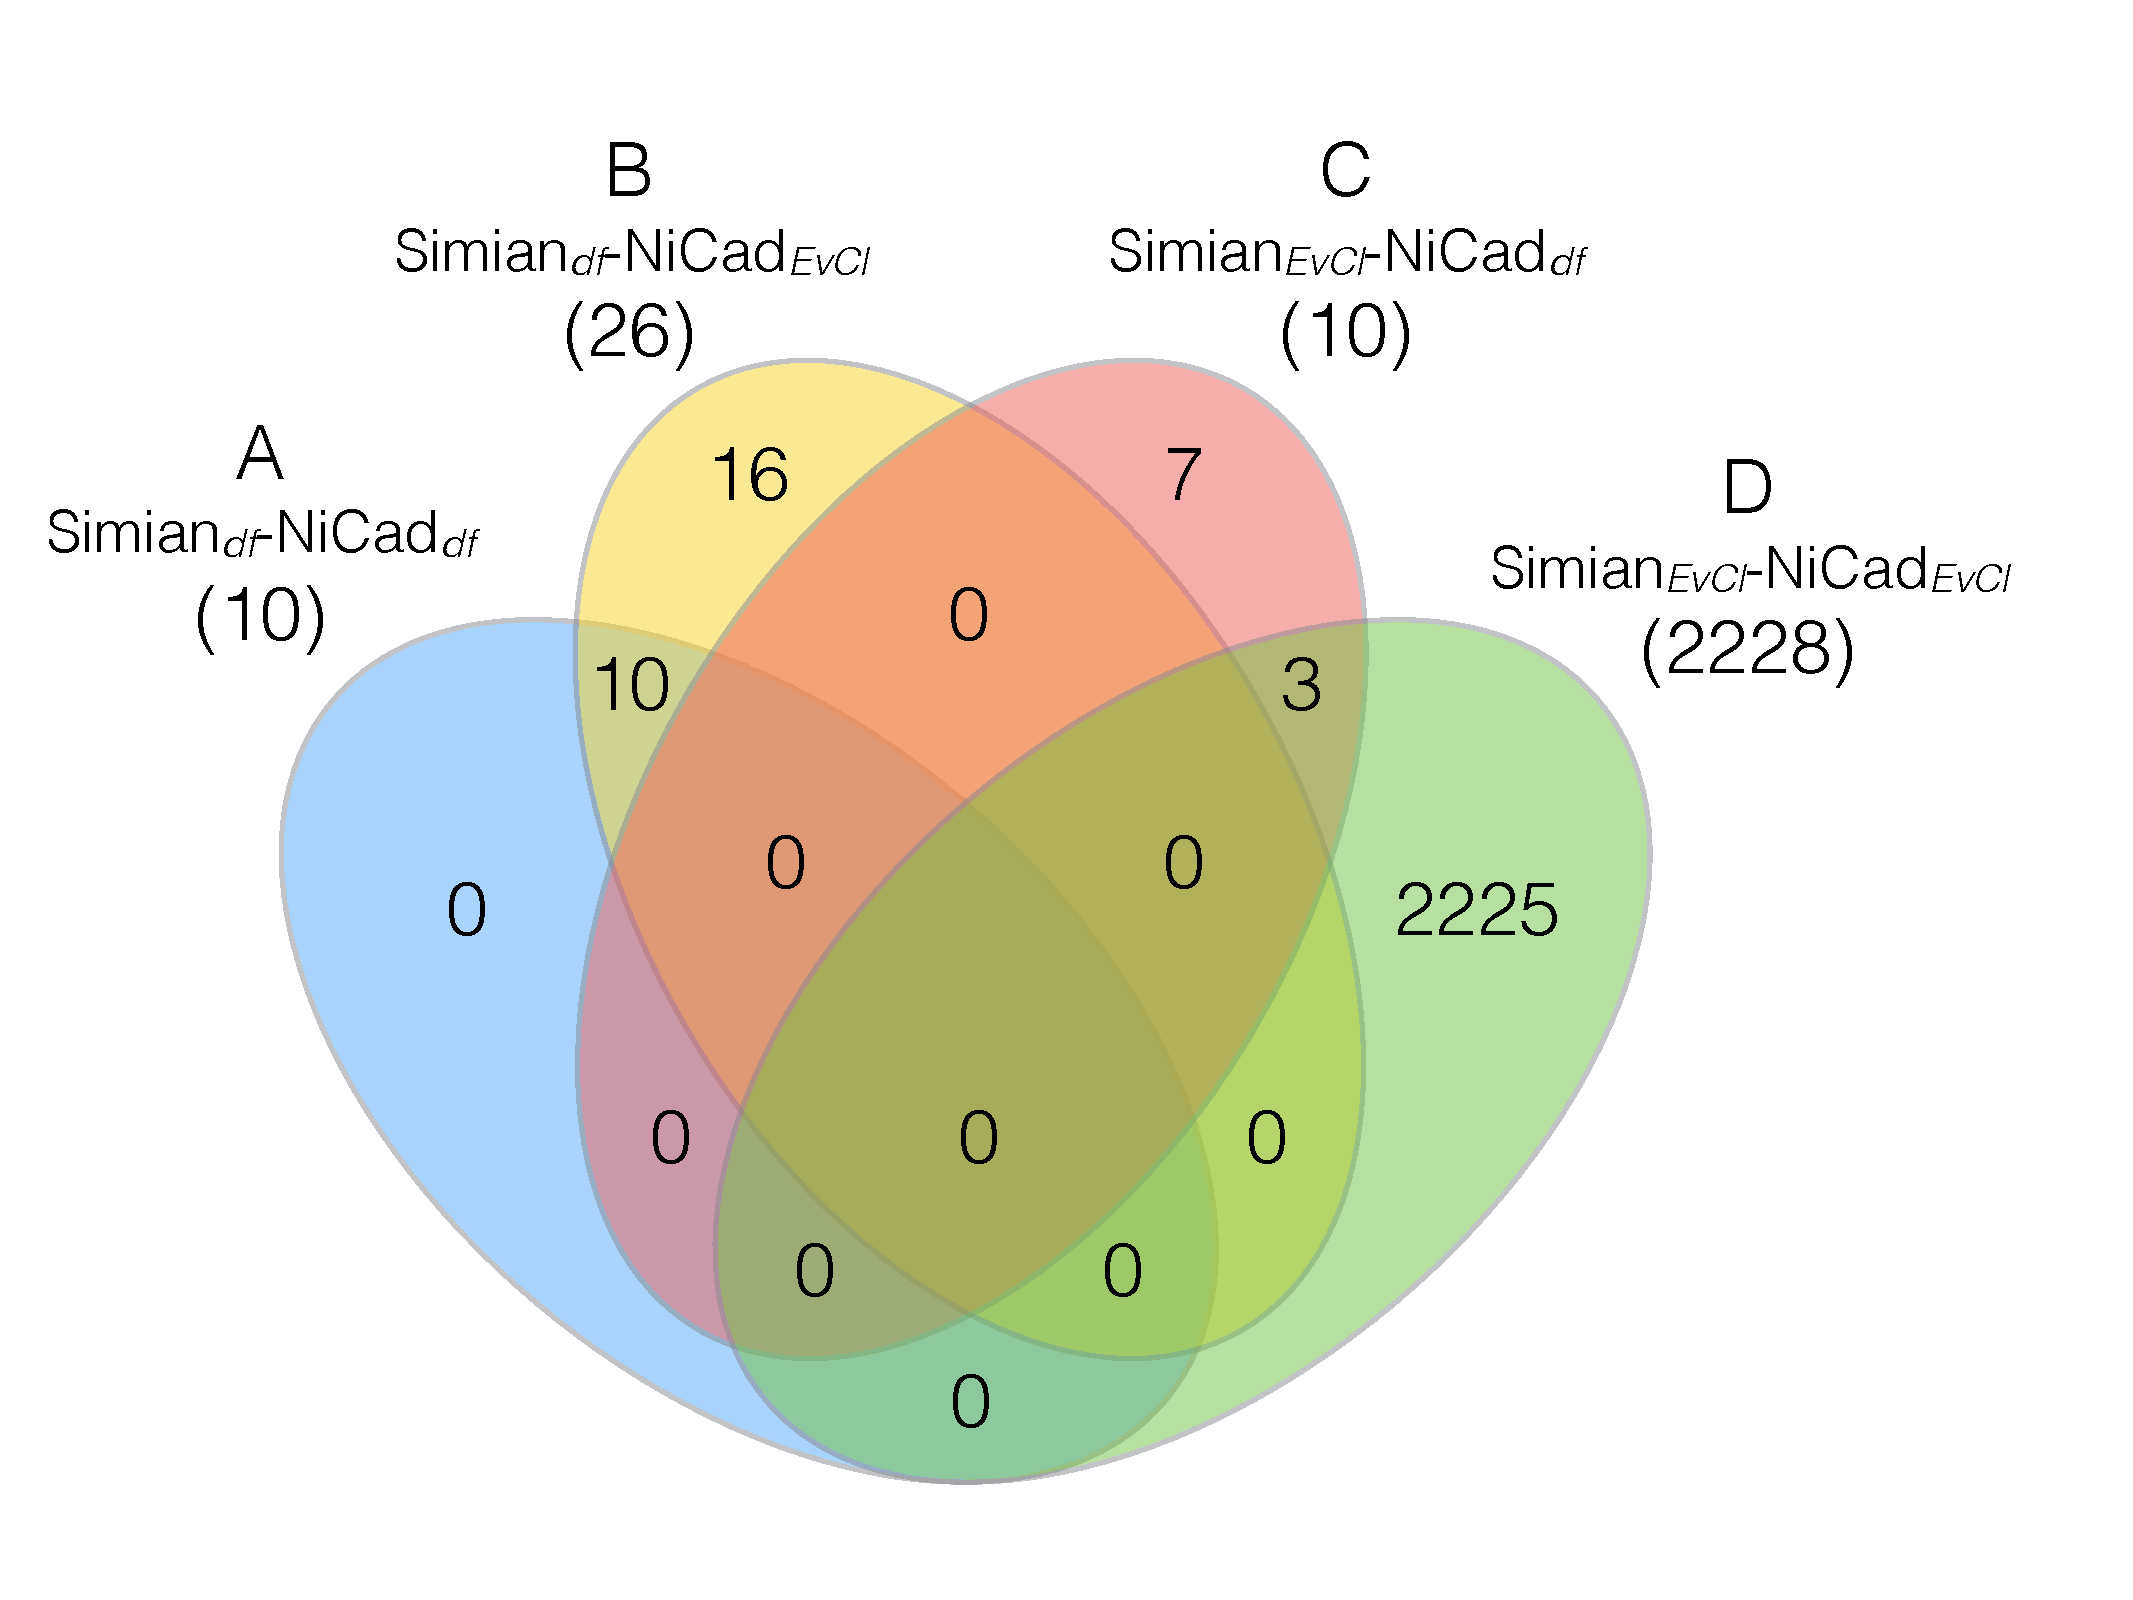
\includegraphics[width=0.8\linewidth]{venn4_pairs_good_pt1+2}
		\caption{Distributions of good-match(0.7) pairs}
		\label{fig:venn4_orig_good}
	\end{minipage}
	\begin{minipage}{.5\textwidth}
		\centering
		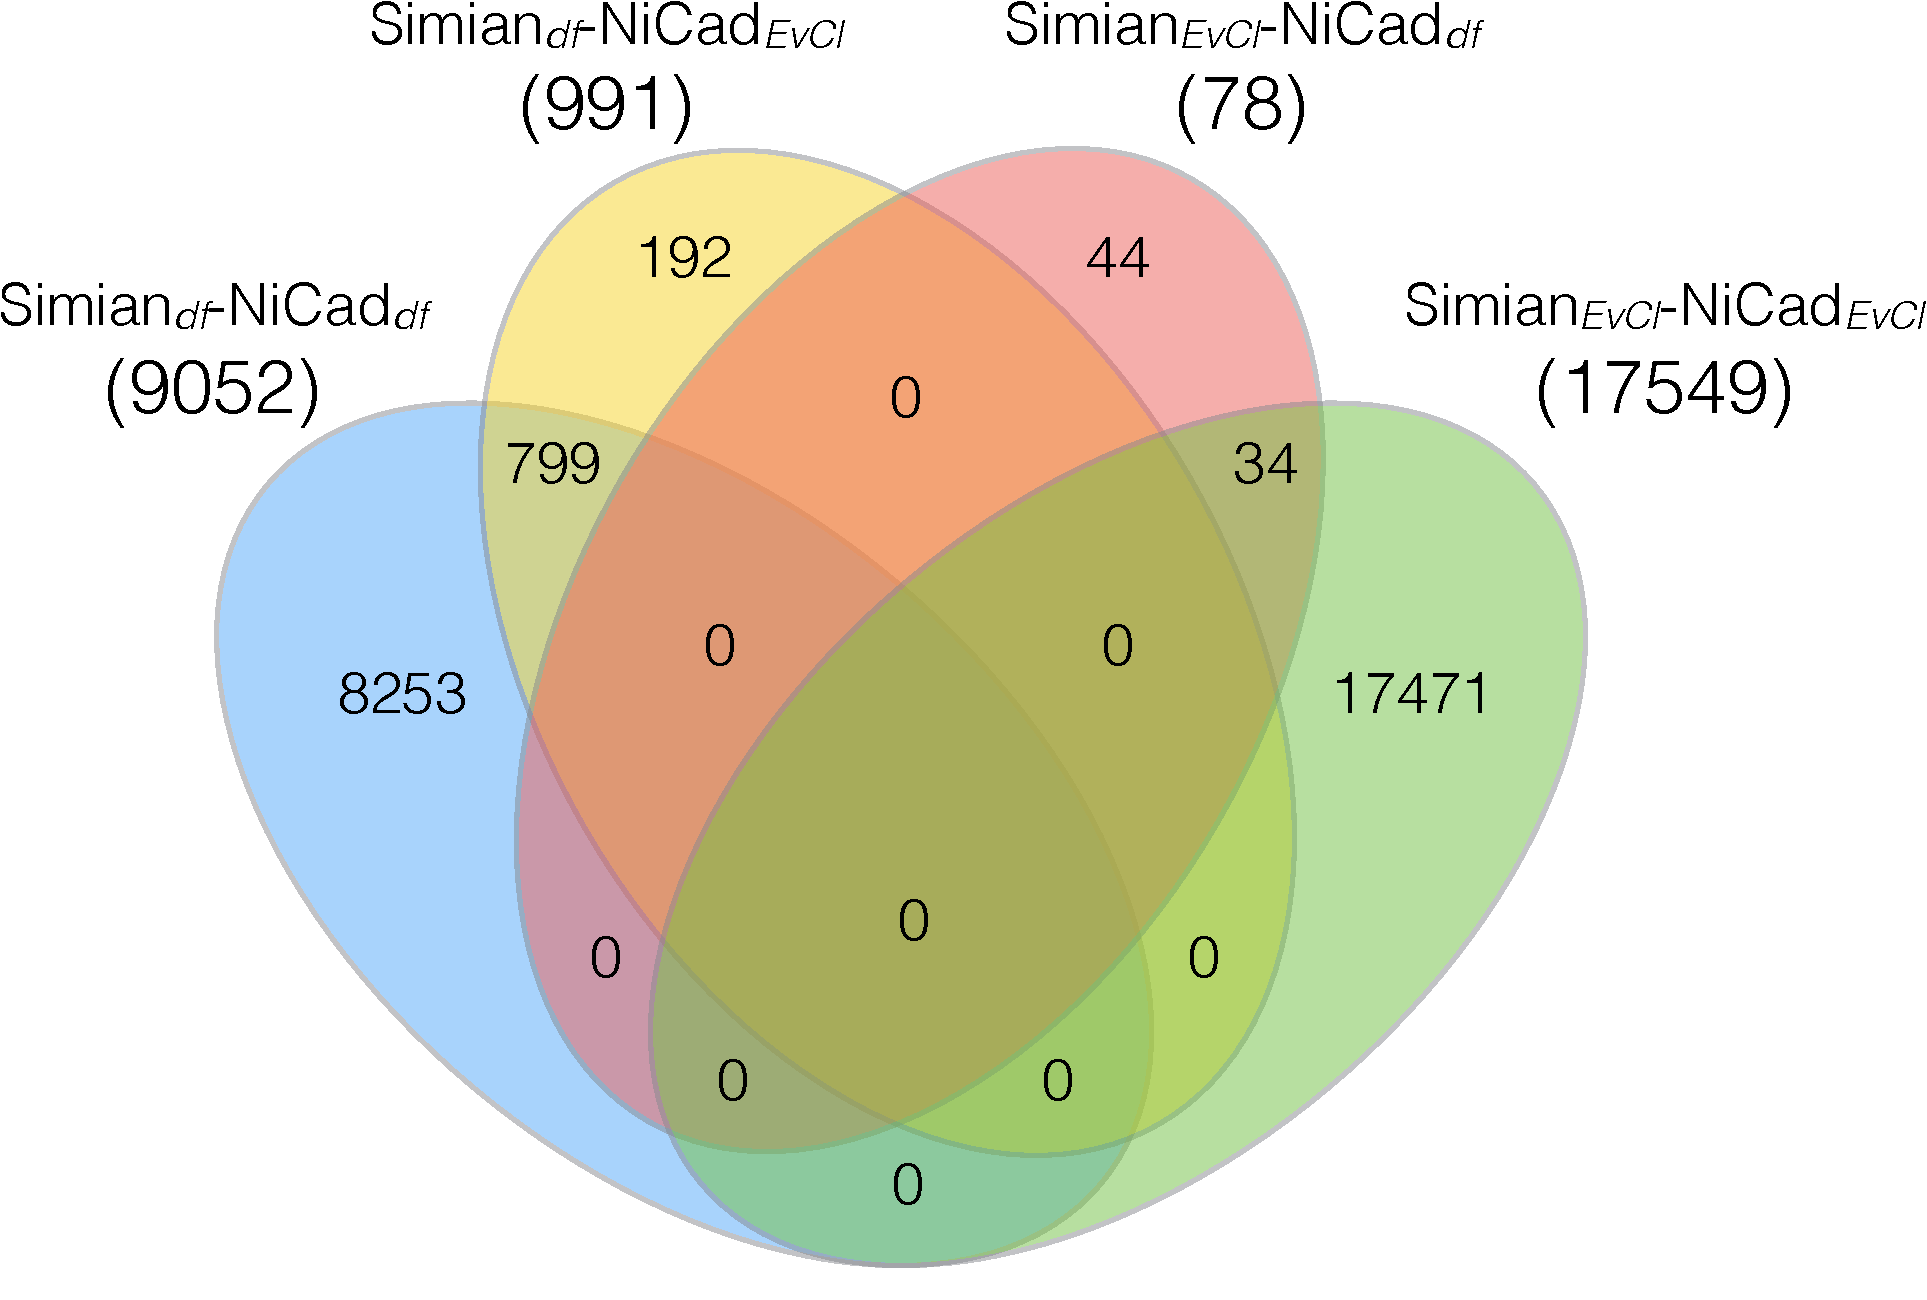
\includegraphics[width=0.8\linewidth]{venn4_pairs_ok_pt1+2+3}
		\caption{Distributions of ok-match(0.7) pairs}
		\label{fig:venn4_orig_ok}
	\end{minipage}
\end{figure*}

\subsubsection{Classifications of online code clones}

\begin{table*}
	\centering
	\caption{Classifications of online code clones}
	\label{tab:classification_scheme}
	\begin{tabular}{|c|p{13cm}|}
		\hline 
		Category & Descriptions \\ 
		\hline 
		A & Code in Stack Overflow is copied from Qualitas (Q $\rightarrow$ S). \\ 
		\hline 
		A' & Code in Qualitas is copied from Stack Overflow (S $\rightarrow$ Q). \\ 
		\hline 
		B & Clone pair is exactly identical or highly similar and may be copied either from each other or a third source (unknown) (S $\leftrightarrow$ Q $\vee$ (T $\rightarrow$ S $\wedge$ T $\rightarrow$ Q)).
		\\ 
		\hline 
		C & Code in both places are copied from a third source T (known) (T $\rightarrow$ S $\wedge$ T $\rightarrow$ Q).
		\\ 
		\hline 
		D & Code is a boiler-plate or IDE auto-generated.
		\\ 
		\hline 
		E & Code in both places initialise a similar/the same object; extend the same class/its subclass; implement the same interface.
		\\ 
		\hline 
		F & Accidental similarity, false clone \\ 
		\hline 
	\end{tabular} 
\end{table*}

We need an appropriate classification scheme to be able to meaningfully manually categorise the selected clone candidates. We adapted the classifications from a study by Kapser et al. \cite{Kapser2006}. The online code clone classification scheme is described in \Cref{tab:classification_scheme}. Due to differences in the experimental settings of the study, we adopted some of the original classifications and added a few more classifications to match with our datasets and context. The final seven categories (A--F) have been observed to be common clone patterns found from a manual check of 100 random sample clone pairs. Category A is a clone pair that has evidence to be copied from Qualitas to Stack Overflow (by having comments in source code and explanation or links in Stack Overflow post), and vice versa in category A'. Category B is a clone pair that is exactly identical or highly similar but without any attribution of copying. Category C is a clone pair that has information confirming of copying but from the same external source. Category D is a clone pair that is either boiler-plate code (e.g. \verb|equals()| methods, or getters and setters) or IDE-generated (e.g. GUI initialisation). Category E are clones created by inheriting the same super class or implementing the same interface. They usually share similar overriding methods. The last category, category F, are false clones that have accidental similarity after code normalisation or other causes. Using this classification scheme, we consider clone pairs in category A, A', B, C as true positive, and clone pairs in category D, E, F as false positive. 

\subsubsection{Manual investigation of agreement-based clone pairs}

The first author who has been working on clone detection research for two years takes the role of an investigator who performs manual investigation. Following the classification scheme, the investigator manually goes through each agreement-based clone pair, looks at the clones, and chooses the most appropriate category for the pair. A relevant and useful observation is also recorded for each clone pair. The classification results are shown in \Cref{tab:classification_good_o}. We have manually investigated 2,261 good-match clone pairs. There is one clone pair found to be copied from a Qualitas project to Stack Overflow, 4 pairs that are highly similar or identical but without any evidence of copying (no comments in neither Stack Overflow post nor Qualitas source code), and 3 pairs that are copied from external sources. The rest are false positive clones. 58 clone pairs are found to \verb|equals()| methods, or getters and setters. Six pairs are similar code from inheritance of the same superclass or implementing the same interface. Finally, 2,189 clone pairs are false clones.

For the ok-match clone pairs, we could not feasibly investigate 23,868 pairs manually.  According to the manual investigation of good-match results, we found that Simian$_{\textrm{\textit{EvCl}}}$--NiCad$_{\textrm{\textit{EvCl}}}$ produces a large number of 2,253 false positive results (accounts for 99.87\% of Simian$_{\textrm{\textit{EvCl}}}$--NiCad$_{\textrm{\textit{EvCl}}}$ clone pairs) due to its recall preference. We thus decided to leave this configuration out of the ok-match manual investigation. There are totally 4,625 ok-match pairs that were investigated. The 49 true positive pairs found are combinations of 8, 33, and 8 clone pairs in category A, B, and C respectively.

We cannot be certain about the direction of copying in the category-B pairs, since there is no solid information of copying. We thus checked the timestamp of each Java file in Qualitas project and compared it to their respective timestamp of Stack Overflow posts. We found that all Stack Overflow posts were created after their respectively Qualitas Java files \FIXME{check again since the dataset is updated}. This means that the copying can only be either (1) from Qualitas to Stack Overflow or (2) from an external source to both Stack Overflow and Qualitas independently. There is no clone pairs found in A' category.

%\textbf{Qualitas-\textbf{N}:} We decided to filter out the agreed clone pairs reported by agreement of Simian$_{\mathrm{\textit{EvCl}}}$--NiCad$_{\mathrm{\textit{EvCl}}}$ altogether due to its large number of false positive. With the remaining 3 agreements, we did manual investigation of agreed ok-match clone pairs from agreements of Simian$_{df}$--NiCad$_{df}$, Simian$_{df}$--NiCad$_{\mathrm{\textit{EvCl}}}$, and Simian$_{\mathrm{\textit{EvCl}}}$--NiCad$_{df}$. We had not done any investigation of good-match since there were no good-match pairs for these 3 agreements. The number of pairs that have been looked at is 6,706 (excluding duplicates). The results are shown in Table.

\begin{table*}
	\centering
	\caption{Classification results of agreement-based and non agreement-based clone pairs. S$_u$ denotes a number of unique Stack Overflow snippets. Q$_u$ and Q$_{up}$ denote a number of unique Qualitas Java files and unique Qualitas projects respectively.}
	\label{tab:classification_good_o}
	\small
	\resizebox{2.1\columnwidth}{!}{%
	\begin{tabular}{|l"r|r|r|r|r|r|r|r"r|r|r|r|r|r|r"r|r|r|r|}
		\hline
		Classificaiton & A & A' & B & C & \textbf{Sum} & S$_{u}$ & Q$_u$ & Q$_{up}$ & D  & E & F & \textbf{Sum} & S$_{u}$ & Q$_u$ & Q$_{up}$ & \textbf{Total}  & S$_{u}$ & Q$_u$ & Q$_{up}$\\ 
		\hline 
		\hline
		\multirow{1}{*}{\textit{good-match(0.7)}}  & 1 & 0 & 4  & 3 & \textbf{8} & 7 & 6 & 6 & 58  & 6 & 2189 & \textbf{2253} & 81 & 693 & 58 & \textbf{2261} & 87 & 699 & 59 \\
		\multirow{1}{*}{\textit{ok-match(0.7)}}  & 8 & 0 & 29  & 10 & \textbf{47} & 12 & 14 & 10 & 9158 & 35 & 82 & \textbf{9275} & 100 & 204 & 30 & \textbf{9322} & 112 & 218 & 35 \\
		\hline 
		\hline 
		\multirow{1}{*}{\textit{Simian$_{df}$}} & 19 & 0 & 336 & 17 & \textbf{432} & 148 & 229 & 38 & 209 & 63 & 167 & \textbf{439} & 136 & 214 & 49 & \textbf{871} & 271 & 428 & 58 \\
		\hline
		\multirow{1}{*}{\textit{NiCad$_{df}$}} & 8  & 0 & 27 & 1 & \textbf{36} & 16 & 15 & 5 & 77 & 3 & 82 & \textbf{132} & 52 & 55 & 17 & \textbf{168} & 67 & 69 & 19 \\ 
		\hline
	\end{tabular} 
	}
\end{table*}

\subsection{Non agreement-based clone pairs}
%In the preliminary stage of our experiment, we found that there are 41 Stack Overflow fragments reported by Simian with default configurations. However, only 10 of them appear in the new results using tool's agreement. Thus, we further investigated the clone pairs reported by Simian and NiCad but \textit{without} an agreement. 

The non agreement-based clone pairs are clone pairs that are reported by a single tool (either Simian or NiCad) and do not have agreement with another tool. The disagreement can be from misalignment of clone lines or different configurations that results in different clones reported. They are also clone pairs in projects that have NiCad's errors (6 projects for \textit{df} and 27 for \textit{EvCl}). With the four configuration combinations, we decided to investigate only two, Simian$_{df}$, and NiCad$_{df}$, and drop Simian$_{\mathrm{\textit{EvCl}}}$ and NiCad$_{\mathrm{\textit{EvCl}}}$ due to their enormous amount of clone pairs (59 millions and 206 millions respectively). They also have a high possibility of containing a large number of false positives due to relaxation of EvaClone configurations. 

Even choosing only the default configurations, the number of clone pairs are still very large. We hence apply two pruning filters: (1) clone size and (2) similarity threshold. For the clone size filter, we raise the minimum clone size to 10 line. The clone size filter is applied to Simian clone pairs only since its default configurations consider a minimum of 6 line as clones. On the other hand, a minimum of 10 lines is already a default configuration of NiCad. We found that this filter works well with Simian clone pairs resulting in a manageable amount of 795 clone pairs remaining. Regarding the similarity threshold filter, it is only applied to NiCad clone pairs since Simian does not provide this similarity threshold configuration. We increase the similarity threshold of NiCad clone pairs from 70\% to 80\%. This results in 159 clone pairs remaining. The summary of non agreement-based clone pairs is shown in \Cref{tab:classification_indv_stats}.

For Simian$_{df}$, there were 9,383 clone pairs reported by the tool. Out of 9,383 pairs, 140 of them are the ones found in \textit{ok-}pairs using agreement-based detection. We filtered the results further by removing false positives such as similar \verb|equals()|, \verb|hashCode()| methods, getters and setters out by using regular expression. We managed to remove 8,956 pairs using this method. Eventually, there were 287 clone pairs remaining for manual investigation. For NiCad$_{df}$, we obtained 7,040 clone pairs to look at which is infeasible for manual investigation. Hence, result filtering was also needed. However, regular expressions could not be used effectively as in Simian's case since NiCad allowed clones that are different at keywords/variable names or even added/deleted lines. So we decided to filter the results by selecting pairs that pass stricter clone criteria with $\mathrm{UPI} = 0.2$. By reducing the UPI to 0.2, there were totally 166 pairs left. Out of 166, 52 are ok-pairs and 114 are remaining pairs for manual check (18 pairs are from \textit{cayenne} and \textit{iReport} that could not be analysed using UPI = 0.3). The statistics of the clones and classification results are reported in \Cref{tab:classification_indv_stats}.

%We selected only Stack Overflow fragment and Qualitas files that have never been looked at before in the previous investigation. If many clone pairs having the same Stack Overflow fragment and Qualitas file, we keep only the largest one. The reason for having this criteria is that we found a lot of duplicate clone pairs with the same classifications from either Stack Overflow fragments or Qualitas files. The classification results are shown in Table \ref{tab:classification_indv}. 

\begin{table}
	\centering
	\caption{Statistics of non-agreed clone pairs (Simian$_{df}$ and NiCad$_{df}$).}
	\label{tab:classification_indv_stats}
	\small
	\resizebox{\columnwidth}{!}{%
	\begin{tabular}{l|p{2.4cm}|r|r|r}
		\hline 
		Tool & Filter & C$_{\textrm{\textit{pairs}}}$ & good/ok & remaining \\ 
		%\hline 
		%\multirow{1}{*}{\textit{Simian$_{df}$}-1} & 9383 & 140 & 8951 & 292 \\
		%\multirow{1}{*}{\textit{Simian$_{df}$}-2} & 9042 & 0 & 8539 & 503 \\
		\hline
		\multirow{1}{*}{\textit{Simian$_{df}$}} & $minline \geq 10$ \newline reg.~expressions & 67570 & 2546 & 871 \\ %140 + 1482 + 926
		\hline
%		\multirow{1}{*}{\textit{NiCad$_{df}$}-1} & 7040  & 226 & 6700 & 114 \\
%		\multirow{1}{*}{\textit{NiCad$_{df}$}-2} & 22187  & 152 & 21990 & 45 \\
		\multirow{1}{*}{\textit{NiCad$_{df}$}} & $similarity \geq 80\%$ & 229176  & 450 & 168 \\
		\hline
	\end{tabular} %
	}
\end{table}

\subsubsection{Manual investigation of non-agreed clone pairs}
%\subsubsection*{\textbf{Qualitas-\textit{O} (v. 2013-09-01r)}}
We performed manual investigation and classified the clone pairs reported by Simian$_{df}$ and NiCad$_{df}$ in the same way as the agreement-based clone pairs. The results of the manual investigation is reported in \Cref{tab:classification_good_o}.

%\subsection{Summary of true online clone pairs}
\begin{table}[H]
	\centering
	\caption{Numbers of true positive online clone pairs found by manual investigation}
	\label{tab:classification_true_pairs_summary}
	\small
	\begin{tabular}{l|r|r|r|r|r}
		\hline 
		Tool & A & A' & B & C & Total \\
		\hline
		good-pairs & 1 & 0 & 4 & 3 & 8 \\
		ok-pairs & 8 & 0 & 29 & 10 & 47 \\
		Simian$_{df}$ pairs & 79 & 0 & 336 & 17 & 432 \\
		NiCad$_{df}$ pairs & 8 & 0 & 27 & 1 & 36 \\
		\hline 
		Total & 96 & 0 & 396 & 31 & 523 \\
		\hline
	\end{tabular} 
\end{table}

\begin{figure}
	\centering
	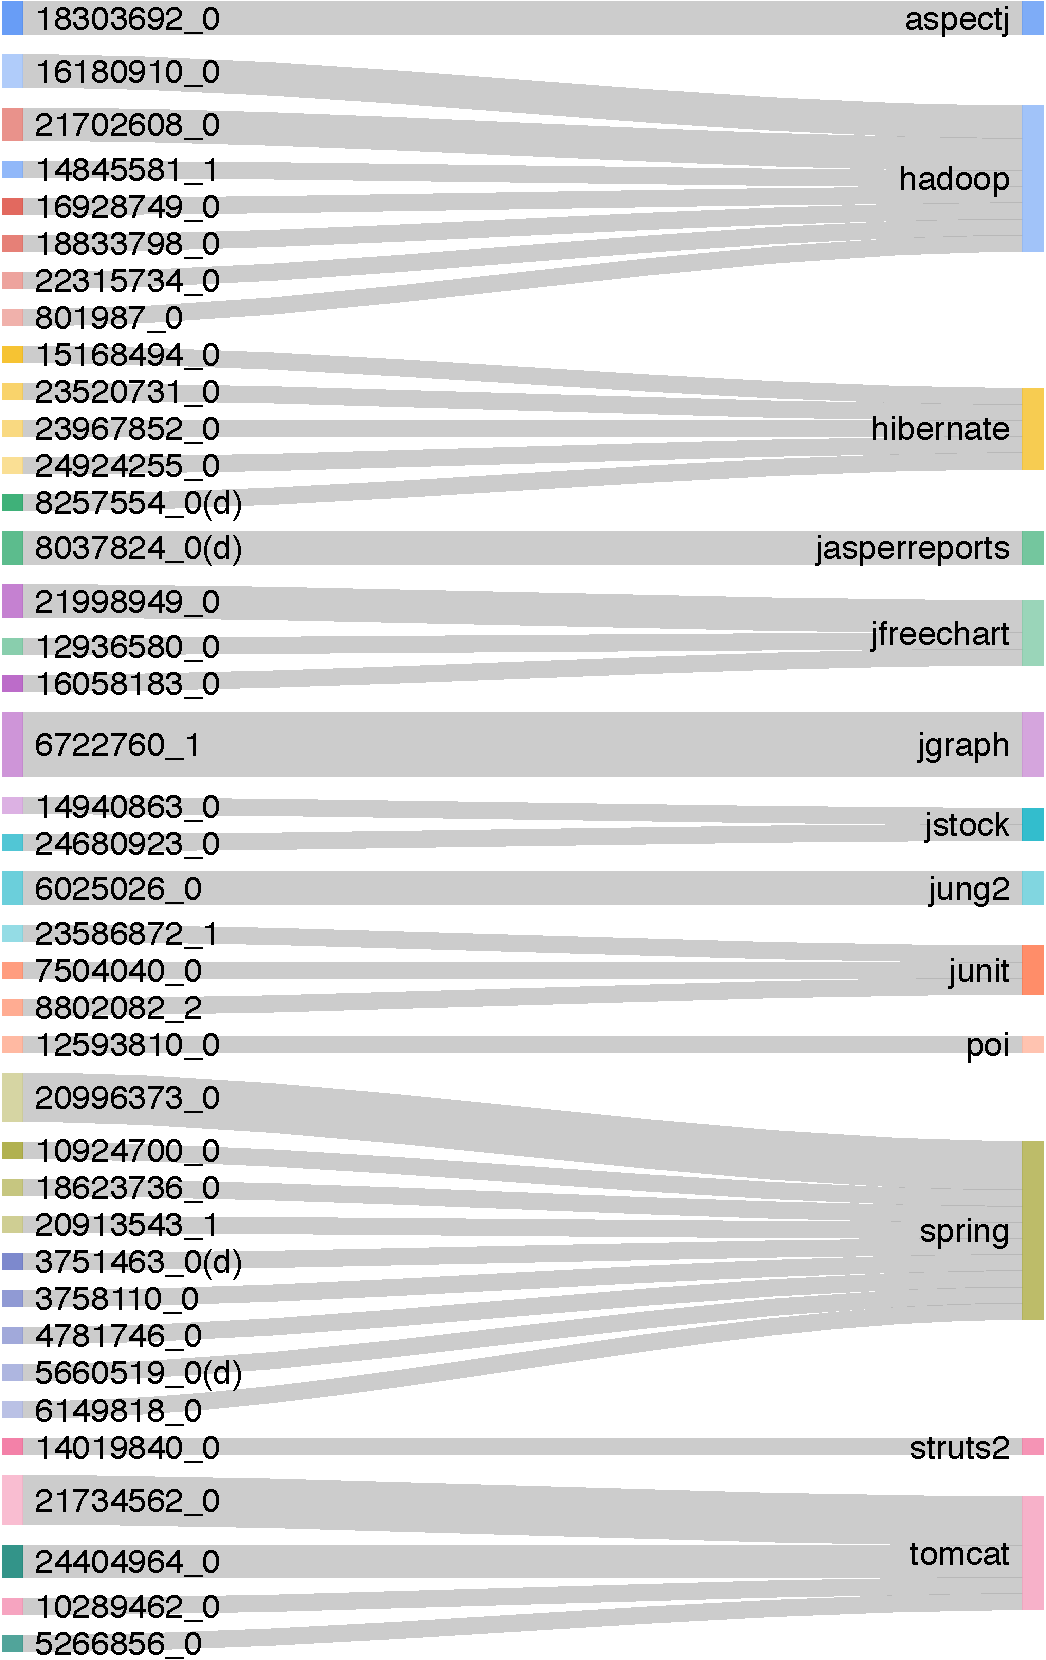
\includegraphics[width=\linewidth]{Sankey_proj}
	\caption{Relationships of 58 Stack Overflow clone pairs to their original projects. 55 are outdated and 3 are deleted (shown using (d) suffix).}
	\label{fig:sankey}
\end{figure}

%\subsubsection{Qualitas-\textit{N} (v. 2016-08-05)}

\section{Effects of online code clone}

In this study, we are interested in the effects of online code clones to software development. From the manual investigation of 184 true online clone pairs, we found that there are two potential issues: stale online code, and software licensing violation.

\subsection{Issue~1 -- stale online code clones}
Stale online code occurs when a piece of code has been copied from a software project to Stack Overflow, and later it has been changed in the original project. However, in this situation, the copy is still unchanged. Since the code were updated due to various possible reasons including bug fixing, this can cause a problem if developers reuse stale online code from Stack Overflow. They might also introduce the same unfixed bug(s) into the software. To discover stale online code, we focus on the true online clone pairs that are copied in the direction from Qualitas to Stack Overflow (category-\textit{A} online clone pairs) in \Cref{tab:classification_true_pairs_summary} which results in 84 pairs selected. %We restricted it further to only the ones having versioning system so we can trace changes made to these clone pairs. Fortunately, all of the pairs were from projects with either git or svn so we did not remove any pair from this set. 

%Our intuition behind his issue comes from a situation where a piece of code has been copied from a Qualitas project and posted on Stack Overflow. Later, that piece of code has been modified further to accommodate changes in the projects (or any other reasons). However, even the code in Qualitas project is already updated, the one posted on Stack Overflow is not changed. This results in outdated online code which can cause problems when programmers copy and use it in their projects.

%We decided to ignore NiCad results from this analysis due to its failure of clone clustering and renaming on some projects.  Thus, the 39 projects are the ones that can be analysed by Simian, have newer versions than the versions in Qualitas-\textit{O}, and have code version control system (either git or svn). %After filtering, there are 141 pairs removed because 45 of them do not have new versions (7 from c-jdbc, 21 from Compiere, 7 from heritrix, and 10 from iReport) and 4 of them we could not find source code with version control (2 from findbugs, 1 from jag, and 1 from jgraphpad). Finally there were 134  pairs remaining. %We are interested in clone pairs that were changed after they appeared on Stack Overflow.

\Cref{tab:stale_code} shows the results of manual investigation of 84 category-A online clone pairs. The investigation reveals that there are 50 clone pairs that are outdate (i.e. ``stale clone''). They are clone pairs that were copied from Qualitas projects to Stack Overflow and marked as accepted answers, and later have been changed during the development.  

\begin{table}
	\centering
	\caption{Results from a manual investigation of 84 category-A online clone pairs}
	\label{tab:stale_code}
	\small
%	\resizebox{\columnwidth}{!}{%
	\begin{tabular}{l|r|r|r|r|r}
		\hline 
		Project & Pairs & Stale & Fresh & Del. & Others \\
		\hline
		ant & 1 & 0 & 1 & 0 & 0 \\
		log4j & 4 & 0 & 4 & 0 & 0 \\
		tomcat & 7 & 7 & 0 & 0 & 0 \\
		aspectj & 2 & 2 & 0 & 0 & 0 \\
		eclipse-SDK & 12 & 5 & 7 & 0 & 0 \\
		hadoop & 14 & 9 & 5 & 0 & 0 \\
		hibernate & 16 & 4 & 11 & 1 & 0 \\
		jasperreports & 2 & 2 & 0 & 0 & 0 \\
		jfreechart & 4 & 4 & 0 & 0 & 0 \\
		jgraph & 5 & 4 & 0 & 0 & 1 \\
		jgrapht & 1 & 0 & 1 & 0 & 0 \\
		jstock & 2 &  2 & 0 & 0 & 0 \\
		jung & 2 & 2 & 0 & 0 & 0 \\
		junit & 3 & 3 & 0 & 0 & 0 \\
		poi & 3 & 1 & 2 & 0 & 0 \\
		spring & 14 & 9 & 3 & 2 & 0 \\
		struts & 1 & 1 & 0 & 0 & 0 \\
		weka & 3 & 0 & 3 & 0 & 0 \\
		\hline
		Total & 96 & 55 & 37 & 3 & 1 \\
		\hline
	\end{tabular} 
%}
\end{table}

\begin{table*}
	\centering
	\caption{58 code clones in Stack Overflow that were altered, rewritten, or removed from the project after posted and their respective licenses}
	\label{tab:stale_code_details}
	\small
	\resizebox{2.1\columnwidth}{!}{%
	\begin{tabular}{r|l|l|l|l|c|l}
		\hline 
		No. & Project & File & License & SO Post & Changes & Date \\
		\hline
			1 & aspectj-1.6.9  & Agent.java  & -- & 18303692 & alteration  & 2015-09-08 \\
			2 & aspectj-1.6.9  & Agent.java  & -- & 18303692 & alteration  & 2015-09-08 \\
			3 & eclipse-SDK  & GenerateToStringAction.java  & EPLv1 & 2513183 & alteration  &  2015-03-17 \\
			4 & eclipse-SDK  & GenerateToStringAction.java  & EPLv1  &  2513183	 & alteration  &  2015-03-17 \\
			5 & eclipse-SDK  & GenerateToStringAction.java  & EPLv1  &  2513183	 & alteration  &  2015-03-17 \\
			6 & eclipse-SDK  & GenerateToStringAction.java  & EPLv1  &  2513183	 & alteration  & 2011-03-01 \\
			7 & eclipse-SDK  & WizardDialog.java  & EPLv1  &   11861598	 & alteration  &  2011-02-03 \\
			8 & hadoop-1.0.0  & DBCountPageView.java  & Apache-2 & 21702608 & alteration  & 2011-06-12 \\
			9 & hadoop-1.0.0  & DBCountPageView.java  & Apache-2 & 21702608 & alteration  & 2011-06-12 \\
			10 & hadoop-1.0.0  & JobSubmissionFiles.java  & Apache-2 & 14845581 & alteration  & 2012-06-25 \\
			11 & hadoop-1.0.0  & LineRecordReader.java  & Apache-2 & 16180910 & alteration  & 2011-07-25 \\
			12 & hadoop-1.0.0  & LineRecordReader.java  & Apache-2 & 16180910 & alteration  & 2011-07-25 \\
			13 & hadoop-1.0.0  & StringUtils.java  & Apache-2 & 801987 & alteration  & 2013-02-04 \\
			14 & hadoop-1.0.0  & TestJobCounters.java  & Apache-2 & 18833798 & alteration  & 2011-06-12 \\
			15 & hadoop-1.0.0  & TextOutputFormat.java  & Apache-2 & 16928749 & alteration  & 2011-06-12 \\
			16 & hadoop-1.0.0  & WritableComparator.java  & Apache-2 & 22315734 & alteration  & 2014-11-20 \\
			17 & hibernate-4.2.2  & ConnectionProviderInitiator.java  & -- & 15168494 & alteration  & 2012-06-24 \\
			18 & hibernate-4.2.2  & Example.java  & -- & 24924255 & alteration  & 2013-04-23 \\
			19 & hibernate-4.2.2  & SchemaUpdate.java  & -- & 23520731 & alteration  & 2016-02-05 \\
			20 & hibernate-4.2.2  & SettingsFactory.java  & -- & 8257554 & removal  & 2011-03-11 \\
			21 & hibernate-4.2.2  & SQLServer2005LimitHandler.java  & -- & 23967852 & alteration  & 2015-03-12 \\
			22 & jasperreports-3.7.4  & JRVerifier.java  & GLGPLv3+ & 8037824 & alteration  & 2008-04-17 \\
			23 & jasperreports-3.7.4  & JRVerifier.java  & GLGPLv3+ & 8037824 & alteration  & 2011-05-20 \\
			24 & jfreechart-1.0.13  & AbstractXYItemRenderer.java  & GLGPLv2.1+ & 12936580 & alteration  & 2016-02-19 \\
			25 & jfreechart-1.0.13  & KeyToGroupMap.java  & GLGPLv2.1+ & 16058183 & alteration  & 2013-07-03 \\
			26 & jfreechart-1.0.13  & SpiderWebPlot.java  & GLGPLv2.1+ & 21998949 & alteration  & 2008-06-02 \\
			27 & jfreechart-1.0.13  & SpiderWebPlot.java  & GLGPLv2.1+ & 21998949 & alteration  & 2008-06-02 \\
			28 & jgraph-5.13.0.0  & HelloWorld.java  & GLGPLv2.1+ & 6722760 & rewriting  & 2014-04-13 \\
			29 & jgraph-5.13.0.0  & HelloWorld.java  & GLGPLv2.1+ & 6722760 & rewriting  & 2014-04-13 \\
			30 & jgraph-5.13.0.0  & HelloWorld.java  & GLGPLv2.1+ & 6722760 & rewriting  & 2014-04-13 \\
			31 & jgraph-5.13.0.0  & HelloWorld.java  & GLGPLv2.1+ & 6722760 & rewriting  & 2014-04-13 \\
			32 & jstock-1.0.7c  & GoogleMail.java  & GPLv2+ & 14940863 & alteration  & 2015-12-13 \\
			33 & jstock-1.0.7c  & GoogleMail.java  & GPLv2+ & 24680923 & alteration  & 2015-12-13 \\
			34 & jung2-2\_0\_1  & ShortestPathDemo.java  & -- & 6025026 & alteration  & 2010-04-13 \\
			35 & jung2-2\_0\_1  & ShortestPathDemo.java  & -- & 6025026 & alteration  & 2010-04-13 \\
			36 & junit-4  & Assert.java  & -- & 23586872 & alteration  & 2015-05-12 \\
			37 & junit-4  & ExternalResource.java  & -- & 7504040 & alteration  & 2016-06-25 \\
			38 & junit-4.11  & ExpectException.java  & -- & 8802082 & alteration  & 2014-05-26 \\
			39 & poi-3.6-20091214  & WorkbookFactory.java  & Apache-2 & 12593810 & alteration  & 2015-04-29 \\
			40 & spring-framework-3.0.5  & AnnotationMethodHandlerExceptionResolver.java  & Apache-2 & 5660519 & removal  & 2012-01-20 \\
			41 & spring-framework-3.0.5  & AutowireUtils.java  & Apache-2 & 20913543 & alteration  & 2014-10-28 \\
			42 & spring-framework-3.0.5  & CustomCollectionEditor.java  & Apache-2 & 18623736 & alteration  & 2013-11-21 \\
			43 & spring-framework-3.0.5  & DefaultAnnotationHandlerMapping.java  & Apache-2 & 3758110 & removal  & 2012-01-20 \\
			44 & spring-framework-3.0.5  & DefaultPropertiesPersister.java  & Apache-2 & 6149818 & alteration  & 2013-03-19 \\
			45 & spring-framework-3.0.5  & DelegatingServletInputStream.java  & Apache-2 & 20996373 & alteration  & 2016-07-15 \\
			46 & spring-framework-3.0.5  & DelegatingServletInputStream.java  & Apache-2 & 20996373 & alteration  & 2008-12-18 \\
			47 & spring-framework-3.0.5  & DelegatingServletInputStream.java  & Apache-2 & 20996373 & alteration  & 2008-12-18 \\
			48 & spring-framework-3.0.5  & DispatcherServlet.java  & Apache-2 & 4781746 & alteration  & 2011-08-08 \\
			49 & spring-framework-3.0.5  & Jaxb2Marshaller.java  & Apache-2 & 10924700 & alteration  & 2012-08-28 \\
			50 & spring-framework-3.0.5  & ScheduledTasksBeanDefinitionParser.java  & Apache-2 & 3751463 & alteration  & 2016-07-05 \\
			51 & struts2-2.2.1  & DefaultActionMapper.java  & Apache-2 & 14019840 & alteration  & 2013-10-18 \\
			52 & tomcat-7.0.2  & BasicAuthenticator.java  & Apache-2 & 21734562 & alteration  & 2016-08-04 \\
			53 & tomcat-7.0.2  & BasicAuthenticator.java  & Apache-2 & 21734562 & alteration  & 2016-08-04 \\
			54 & tomcat-7.0.2  & CoyoteAdapter.java  & Apache-2 & 24404964 & alteration  & 2012-11-18 \\
			55 & tomcat-7.0.2  & CoyoteAdapter.java  & Apache-2 & 24404964 & alteration  & 2012-11-18 \\
			56 & tomcat-7.0.2  & FormAuthenticator.java  & Apache-2 & 21734562 & alteration  & 2016-08-04 \\
			57 & tomcat-7.0.2  & HttpServlet.java  & Apache-2 & 5266856 & alteration  & 2011-10-22 \\
			58 & tomcat-7.0.2  & JspRuntimeLibrary.java  & Apache-2 & 10289462 & alteration  & 2012-09-12 \\
		\hline& 
	\end{tabular} %
}
\end{table*}

\subsection{Issue~3 -- external clones}

\subsection{Issue~2 -- software licensing violations}
Software licensing is a paramount factor in software development. Violation of software license can cause a major impact to the delivery of the software and also lead to legal issues. It is an emerging area that software engineering research community is paying attention to. For example, there are studies of automatic technique to identify software licensing from source code files \cite{German2010} and the evolution of licenses in open source projects \cite{DiPenta2010}.

In our study, we reveal another possible situation of software licensing issue caused by code cloning to Stack Overflow. We found that there are at least 84 pieces of code have been copied from 13 open source projects in Qualitas dataset to Stack Overflow as examples. They are also marked as accepted answers which increase their probability of being reused. These 13 open source projects come with their respective software licenses. However, the licensing information are mostly missing from these clones when they are posted on Stack Overflow. Mostly one or a few methods from the full source file are cloned. This makes the license information at the top of the file mostly left uncopied. If developers copy and reuse these pieces of code in their projects, a licensing conflict can quietly happen without realisation of the developers. 

%\section{Investigation of Missing A/B Clone Pairs Reported by Simian$_{df}$}
%We investigated the 41 clone pairs previously reported by Simian with default configurations and manually investigated. The 41 pairs were searched for in 4 new results sets: Simian$_{df}$, Simian$_{\mathrm{\textit{EvCl}}}$, NiCad$_{df}$, NiCad$_{\mathrm{\textit{EvCl}}}$. The investigation results are shown in Table \ref{tab:search}.
%
%\begin{table}
%	\centering
%	\caption{Results of matching the original 41 Simian(default) pairs in the pretty-printed result sets}
%	\label{tab:search}
%	\begin{tabular}{l|r|r}
%		\hline 
%		Settings & Found & Not found \\ 
%		\hline 
%		Simian$_{df}$  &  40 & 1* \\ 
%		\hline 
%		Simian$_{\mathrm{\textit{EvCl}}}$ & 0 & 41  \\ 
%		\hline 
%		NiCad$_{df}$  & 17 & 24 \\ 
%		\hline 
%		NiCad$_{\mathrm{\textit{EvCl}}}$ &  24 & 17 \\ 
%		\hline 
%	\end{tabular} 
%\end{table}
%
%The single missing Stack Overflow fragment (19051537\) (denoted by *) is one of the 11 false clones generated by Simian. It is removed from the results of the pretty-printed version because it is an outlier. The rest are missing because of different parameter settings.
%
%\section{Simian's Parameters}
%
%We have carefully investigated the effects of the Simian's parameter \texttt{-balanceSquareBrackets+}. I found that it works in the expected way of handling a pair of brackets (\texttt{[},\texttt{]}) that span over multiple lines. For example, the two code fragments in Figure \ref{fig:two_frags} would match by having \texttt{-balanceSquareBrackets+} enabled. However, the \texttt{-balanceSquareBrackets+} parameter only works on a small testing environment having toy programs or only small pairs from the full datasets. It does not work with the full complete set of 144,075 Stack Overflow fragments and Qualitas projects. Please find the summary of all the testing scenarios in Table \ref{tab:summary}. %I found that this pair is missing if I turned on \texttt{-balanceSquareBrackets+}.
%
%\noindent\begin{figure*}
%	\scriptsize
%	\begin{lstlisting}[frame=single,style=base]
%	1   public class MagicSquare {                           public class MagicSquare2 {
%	2       private int[][] square;                              @private int[@
%	3       private boolean[] possible;                                      @][@
%	4       private int totalSqs;                                            @] square;@
%	5       private int sum;                                     private boolean[] possible;
%	6       private int numsquares;                              private int totalSqs;
%	7       public static void main ( String[] args ) {          private int sum;
%	8       MagicSquare m = new MagicSquare ( 3 );               private int numsquares;
%	9                                                            public static void main ( String[] args ) {
%	10                                                           MagicSquare m = new MagicSquare ( 3 );
%	\end{lstlisting}
%	\caption{Two identical fragments with only differences in locations of the square brackets. All 7 lines are reported by Simian if \small\texttt{-balanceSquareBrackets+} \normalsize is enabled. If not, the clone pairs is reported as \newline (MagicSquare.java [3,8], MagicSquare2.java [5,10]).} 
%	\label{fig:two_frags}
%\end{figure*}
%
%\begin{table*}
%	\caption{Simian's \texttt{-balanceSquareBrackets+} (\texttt{-bsb+}) is observed to have unpredictable behaviours when running against big datasets. $\textrm{\textit{CP}}_2$ means the reported clone(s) do not contain lines having dislocated brackets ($L_b$) (i.e. $\textrm{\textit{CP}}_2 = \textrm{\textit{CP}}_1 - L_b$).}
%	\label{tab:summary}
%	\centering
%	\small\begin{tabular}{l|p{6cm}|c|c|c}
%		\hline 
%		\multirow{2}{*}{\textbf{Project 1}} & \multirow{2}{*}{\textbf{Project 2}} & \textbf{Dislocated} & \multirow{2}{*}{\textbf{-bsb+}} & \textbf{Clones pair} \\ 
%		& & \textbf{brackets?} & & \textbf{reported} \\
%		\hline
%		\hline
%		\multicolumn{5}{l}{\textit{Only run Simian against the pair}} \\
%		\hline
%		MagicSquare.java & MagicSquare\_exact\_copy.java & no & 0,1 & $\textrm{\textit{CP}}_1$ \\
%		MagicSquare.java & MagicSquare2.java & yes & 0 & $\textrm{\textit{CP}}_2$ \\ 
%		MagicSquare.java & MagicSquare2.java & yes & 1 & $\textrm{\textit{CP}}_1$ \\
%		\hline
%		%\hline
%		%\multicolumn{5}{c}{\textit{Only run Simian against the pair}} \\
%		%\hline
%		stackoverflow/4298836\_0.java & Qualitas/aoisrc281/../ExprModule.java & no & 0 & $\textrm{\textit{CP}}_3$ \\ 
%		stackoverflow/4298836\_0.java & Qualitas/aoisrc281/../ExprModule.java & no & 1 & $\textrm{\textit{CP}}_3$ \\ 
%		stackoverflow/4533682\_1.java & Qualitas/cobertura-1/../TouchCollector.java & no & 0 & $\textrm{\textit{CP}}_4$ \\ 
%		stackoverflow/4533682\_1.java & Qualitas/cobertura-1/../TouchCollector.java & no & 1 & $\textrm{\textit{CP}}_4$ \\ 
%		\hline 
%		\hline
%		\multicolumn{5}{l}{\textit{Run Simian against the complete stackoverflow data and the project}} \\
%		\hline
%		stackoverflow/4298836\_0.java & Qualitas/aoisrc281/../ExprModule.java & no & 0 & $\textrm{\textit{CP}}_3$ \\ 
%		\cellcolor{red!10}stackoverflow/4298836\_0.java & \cellcolor{red!10}Qualitas/aoisrc281/../ExprModule.java & \cellcolor{red!10}no & \cellcolor{red!10}1 & \cellcolor{red!10}-- \\ 
%		\hline
%		stackoverflow/4533682\_1.java & Qualitas/cobertura-1/../TouchCollector.java & no & 0 & $\textrm{\textit{CP}}_4$ \\ 
%		\cellcolor{red!10}stackoverflow/4533682\_1.java & \cellcolor{red!10}Qualitas/cobertura-1/../TouchCollector.java & \cellcolor{red!10}no & \cellcolor{red!10}1 & \cellcolor{red!10}-- \\
%		\hline 
%	\end{tabular} 
%\end{table*}

\section{Threats to Validity}

\section{Related Work}
\begin{itemize}
	\item Stack Overflow
	\begin{itemize}
		\item Code example \cite{Nasehi2012}
		\item Search for code in Stack Overflow \cite{Diamantopoulos2015,Keivanloo2014,Park2014, Stolee2014}
		\item Stack Overflow to help developers \cite{Ponzanelli2013, Ponzanelli2014}
		\item Improving Stack Oveflow \cite{Diamantopoulos2015, Wang2014, Bosu2013}
		\item Developers' behaviours on Stack Overlow \cite{Wang2013, Movshovitz-Attias2013}
	\end{itemize}
	\item Code clones 
		\begin{itemize}
			\item Definition: Baxter et al. \cite{Baxter1998}
			\item Comparison of clone detectors: \cite{Roy2008, Ragkhitwetsagul2016,Svajlenko2014}
			\item NiCad \cite{Roy2008,Cordy}
			\item Simian \cite{simian}
			\item Clone taxonomy \cite{Kapser2003}
			\item Clone evolution \cite{Pate2013,Mondal2011}
			\item Comparing Quality Metrics for Cloned and non cloned Java Methods: A Large Scale Empirical Study \cite{Saini2016}.
		\end{itemize}
	\item Agreement-based Clone Detection
	\begin{itemize}
		\item Bellon's framework \cite{Bellon2007}.
		\item EvaClone \cite{Wang2013}
		\item Hybrid \cite{Funaro2010}
	\end{itemize}
	\item Software licensing
	\begin{itemize}
		\item Code siblings \cite{German2009}, Ninka -- Automatic indification of SW license \cite{German2010}, Evolution of SW licensing \cite{DiPenta2010}
	\end{itemize}

\end{itemize}

\section{Conclusions}
This paragraph will end the body of this sample document.
Remember that you might still have Acknowledgments or
Appendices; brief samples of these
follow.  There is still the Bibliography to deal with; and
we will make a disclaimer about that here: with the exception
of the reference to the \LaTeX\ book, the citations in
this paper are to articles which have nothing to
do with the present subject and are used as
examples only.
%\end{document}  % This is where a 'short' article might terminate

%ACKNOWLEDGMENTS are optional
\section{Acknowledgments}
This section is optional; it is a location for you
to acknowledge grants, funding, editing assistance and
what have you.  In the present case, for example, the
authors would like to thank Gerald Murray of ACM for
his help in codifying this \textit{Author's Guide}
and the \textbf{.cls} and \textbf{.tex} files that it describes.

%
% The following two commands are all you need in the
% initial runs of your .tex file to
% produce the bibliography for the citations in your paper.
\bibliographystyle{abbrv}
\bibliography{sigproc}  

\end{document}
